% TLP2esam.tex / sample pages for TLP
% v2.11, released 6-nov-2002

\documentclass{tlp}
\usepackage{ifthen}
\usepackage{url}
% Remove hyperref for final version!!
% \usepackage[pdftex,colorlinks=false,urlcolor=blue]{hyperref}
\usepackage{swipl}
\usepackage{amssymb}
\usepackage{upgreek}
\usepackage{color}
\usepackage{textcomp}

\usepackage{listings}


\lstset{
  basicstyle=\ttfamily,
  columns=fixed,
  fontadjust=true,
  basewidth=0.5em,
  xleftmargin=0.5em,
  captionpos=b
}

\newcommand{\authornote}[3]{{\color{#2} {\sc #1}: #3}}
\newcommand\jan[1]{\authornote{jan}{red}{#1}}
\newcommand\TODO[1]{\authornote{TODO}{red}{#1}}

\newcommand\cplint{\texttt{cplint}}
\newcommand\cplintonswish{\cplint{} on SWISH}

\usepackage[pdftex]{graphicx}
\DeclareGraphicsExtensions{.pdf,.jpg,.png}
\graphicspath{{figs/}{./}}
\newcommand{\tag}[1]{\texttt{#1}}
\newcommand{\fnurl}[1]{\footnote{\url{#1}}}
\sloppy

\begin{document}
\bibliographystyle{acmtrans}

\title{Web Prolog and the programmable Prolog Web}


\author[T. Lager]
{TORBJ\"ORN LAGER \\
University of Gothenburg\\
\email{lager@ling.gu.se}
}

\pagerange{\pageref{firstpage}--\pageref{lastpage}}
\volume{\textbf{?} (?):}
%\jdate{August 2007}
\setcounter{page}{1}
%\pubyear{2007}

\maketitle
\begin{abstract}
We describe a programming language called \textit{Web Prolog}. We think of it as a \textit{web programming language}, or, more specifically, as a web \emph{logic} programming language. The language is based on Prolog, with a good pinch of Erlang added. We stay close to traditional Prolog, so close that the vast majority of programs in Prolog textbooks will run without modification. Towards Erlang we are less faithful, picking only features we regard as useful in a web programming language, e.g. features that support concurrency, distribution and intra-process communication. In particular, we borrow features that make Erlang into an \textit{actor programming language}, and on top of these we define the concept of a \textit{pengine} -- a programming abstraction in the form of a special kind of actor which closely mirrors the behaviour of a Prolog top-level. On top of the pengine abstraction we develop a notion of \textit{non-deterministic RPC} and the concept of \textit{the Prolog Web}.
\end{abstract}


\begin{keywords}
Prolog, Erlang, SCXML, web programming
\end{keywords}

%\newpage
%\subsection*{Temporary!}
%\tableofcontents
%\newpage

\section{Introduction}

\noindent As a logic programming language, Prolog represents a programming paradigm which at its core is unique and very different from imperative or functional programming languages. Features such as built-in backtracking search, unification and a built-in clause database form the basis for logic-based knowledge representation and reasoning, and support for meta-programming, user-defined operators, a term-expansion mechanism and grammars is also provided. These are the features that underlie Prolog's reputation as a symbolic AI programming language. Also, they are features that Erlang does not support. In this paper, we present Web Prolog -- a language which combines the most important features of Prolog with those of Erlang.

%-- an attempt to ``plug out'' the sequential part from Erlang and ``plug in'' sequential Prolog instead

%\begin{lstlisting}
%ancestor_of(X,Y) :- parent_of(X,Y).
%ancestor_of(X,Z) :- parent_of(X,Y), ancestor_of(Y,Z).
%
%parent_of(X,Y) :- mother_of(X,Y).
%parent_of(X,Y) :- father_of(X,Y).
%
%mother_of(trude, sally).
%
%father_of(tom,sally).
%father_of(tom,erica).
%father_of(mike,tom).
%\end{lstlisting}

The structure of the paper is as follows. The rest of this section justifies the introduction of yet another dialect of Prolog. Section~\ref{sec:browser} presents an IDE for Web Prolog, introduces the notion of a \textit{node}, and describes the interaction between the IDE and a node over a WebSocket sub-protocol. Section~\ref{sec:language} introduces the language of Web Prolog as such and compares it with Erlang. Section~\ref{sec:beyond-erlang} looks closer at the combination of the actor model and the logic programming model, placing a particular focus on non-determinism and backtracking. The notion of a pengine is described in detail, and a notion of non-deterministic RPC is developed. Section~\ref{sec:previous} describes some earlier work, Section~\ref{sec:discussion} provides a discussion, and Section~\ref{sec:summary} summarises and suggests avenues for further work.


\vspace{-2mm}

\subsection{Web Prolog is a Hybrid Programming Language}\label{sec:hybrid}

%\begin{quote}
%\noindent Imagine a dialect of Prolog with actors and mailboxes and send and receive -- the means necessary for powerful concurrent and distributed programming. Alternatively, think of it as a dialect of Erlang with logic variables, backtracking search and a  built-in database of facts and rules -- the means for logic programming, knowledge representation and reasoning. Also, think of it as a web logic programming language. This is what Web Prolog is all about.
%\flushright\textit{Web Prolog -- the elevator pitch}
%\end{quote}
%
%\noindent Prolog is a logic programming language. Based on formal logic, a subject dating all the way back to the antiquity and tried and tested by generations of logicians and philosophers, logic programming forms a paradigm of it own. Even in its pure form, as a set of Horn clauses, Prolog is Turing complete but a number of extra-logical constructs has been added to ensure its usefulness as a general purpose programming language.  

Web Prolog is not only a logic programming language but also an \textit{actor programming language} as it extends Prolog with primitives for spawning processes and sending and receiving messages in the style of Erlang, i.e. constructs that made Erlang such a great language for programming message-passing concurrency and distribution. Provided we can accept using a syntax which is relational rather than functional it turns out that the surface syntax of Prolog can easily be adapted to express them. Since Prolog and Erlang also share many other properties such as dynamic typing, the use of immutable variables, and a reliance on pattern matching and recursion, creating a hybrid between them seems reasonable. Indeed, it allows us to regard Web Prolog either as a new dialect of Prolog, or as a new dialect of Erlang.

\vspace{-2mm}

\subsection{Web Prolog is a Web Programming Language}\label{sec:hybrid}

There are more than a dozen Prolog systems around, and we do not intend to compete with them, or with Erlang for that matter. Although the proposed hybrid between Prolog and Erlang would likely work as a general-purpose language, this is not what we aim for. Instead, as suggested by the first part of its name and in an effort to find new uses for Prolog, we think of Web Prolog as a special-purpose programming language -- as an embedded, sandboxed scripting language for programming the Web with logic and for implementing web-based communication protocols in the style of Erlang.

%Some twenty-five years in the making, the World Wide Web is a formidable success and the biggest distributed programming system ever constructed, and has, over the years, become a key delivery platform for a variety of sophisticated interactive applications in just about any conceivable domain. By rebranding Prolog as a web programming language we intend to make an attempt to ensure Prolog can be used to build a web endowed with logic and reasoning capabilities. 

Web Prolog is an embedded language, designed to be implemented in a host language running in a host environment. We have embedded our Web Prolog proof-of-concept implementation in SWI-Prolog \cite{wielemaker:2011:tplp} but we are convinced it can also be embedded in other Prolog systems, in systems supporting non-Prolog programming languages or knowledge representation languages, and in web browsers through transpilation into JavaScript or compilation into WebAssembly.

Web Prolog is furthermore a sandboxed language, open to the execution of untested or untrusted source code, possibly from unverified or untrusted clients without risking harm to the host machine or operating system. Therefore, Web Prolog does not include predicates for file I/O, socket programming or persistent storage, but must rely on the host environment in which it is embedded for such features.

%\vspace{-0mm}

\section{Running Web Prolog from a Browser}\label{sec:browser}

A proof-of-concept web-based IDE for Web Prolog has been implemented in a combination of HTML, CSS and JavaScript. The IDE is equipped with an editor and a shell. Figure~\ref{fig:swish-first} shows them as they appear in a browser window, with the editor to the left and the shell to the right.

\begin{figure}[h]
    \centering
	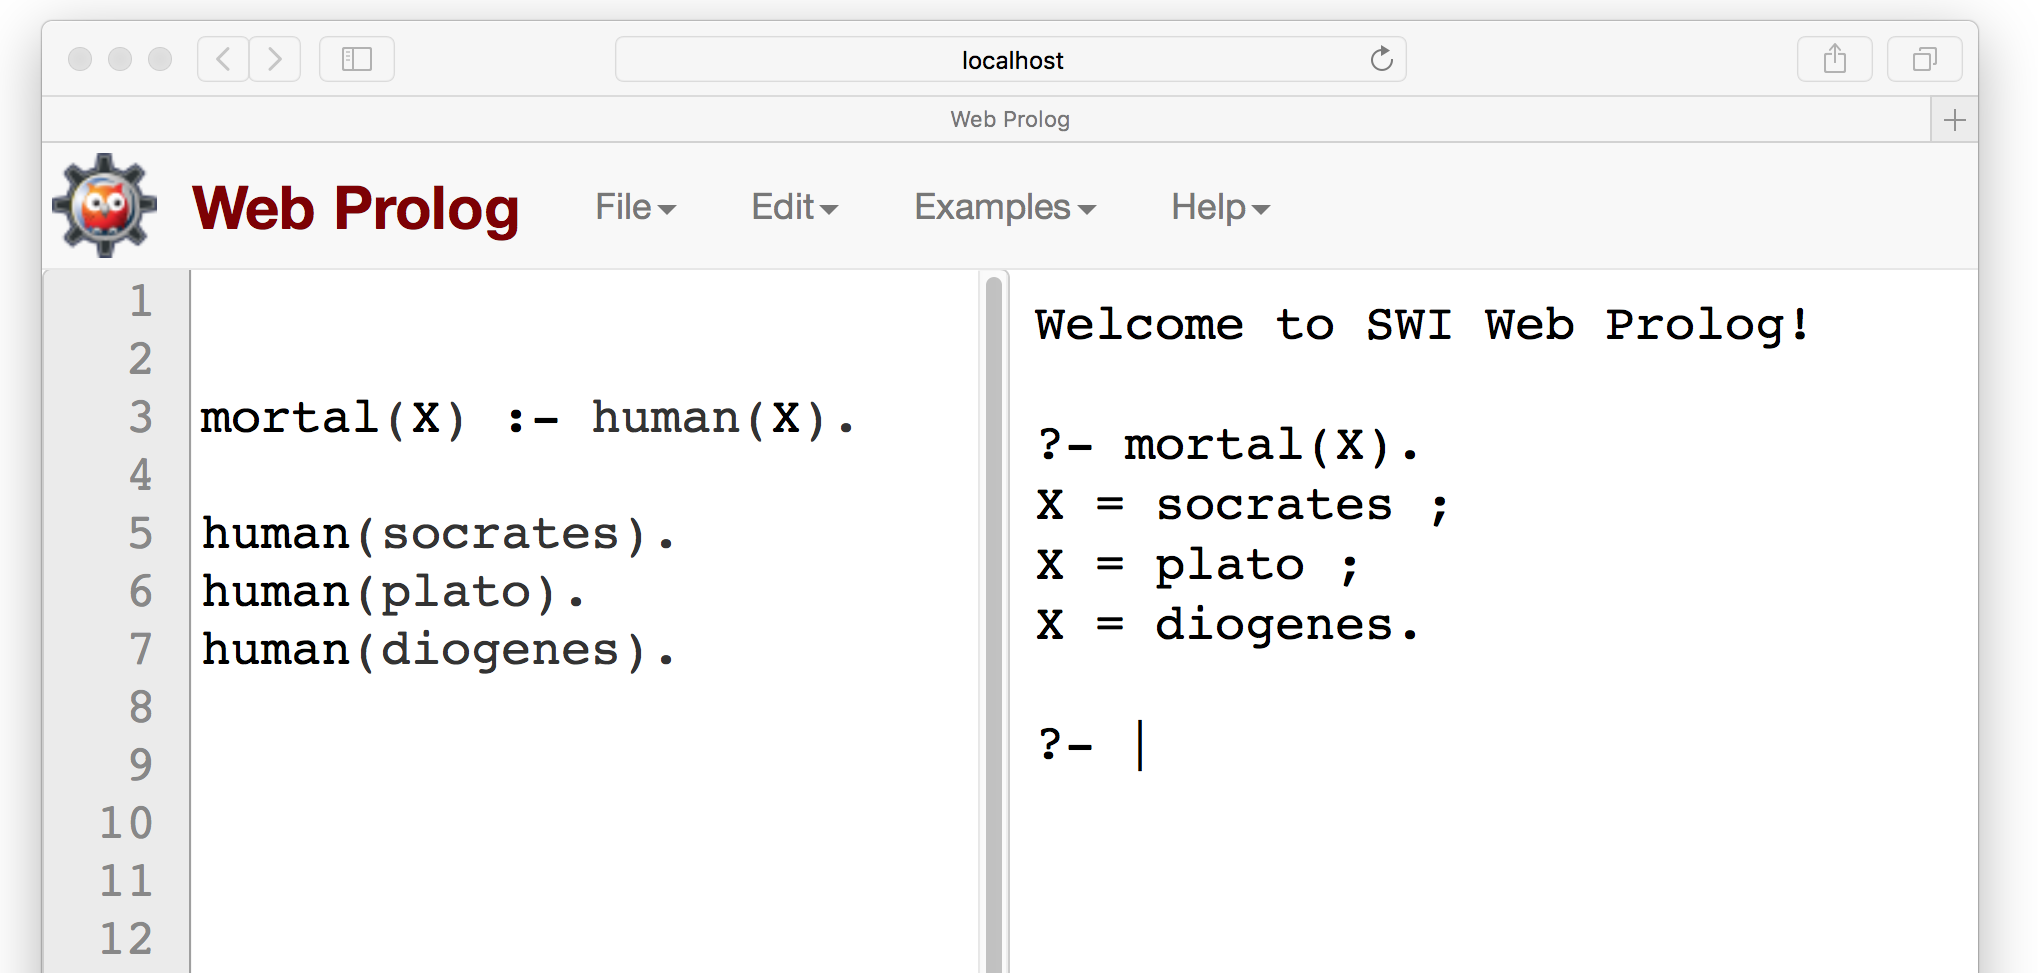
\includegraphics[width=8.7cm]{swish-2}
    \caption{The proof-of-concept IDE.}
    \label{fig:swish-first}
\end{figure}

\noindent The tiny program shown in the editor can be assumed to have been written by a programmer who has then entered a query in the shell in order to inspect the results produced one-at-a-time in the usual lazy fashion typical of interactions with a Prolog top-level. The scenario, depicted in Figure~\ref{fig:swish-pengine-interaction}, also involves a \textit{node}, identified by the URI \texttt{http://local.org}, to which the IDE has established a connection.

%\begin{figure}[h]
%    \centering
%	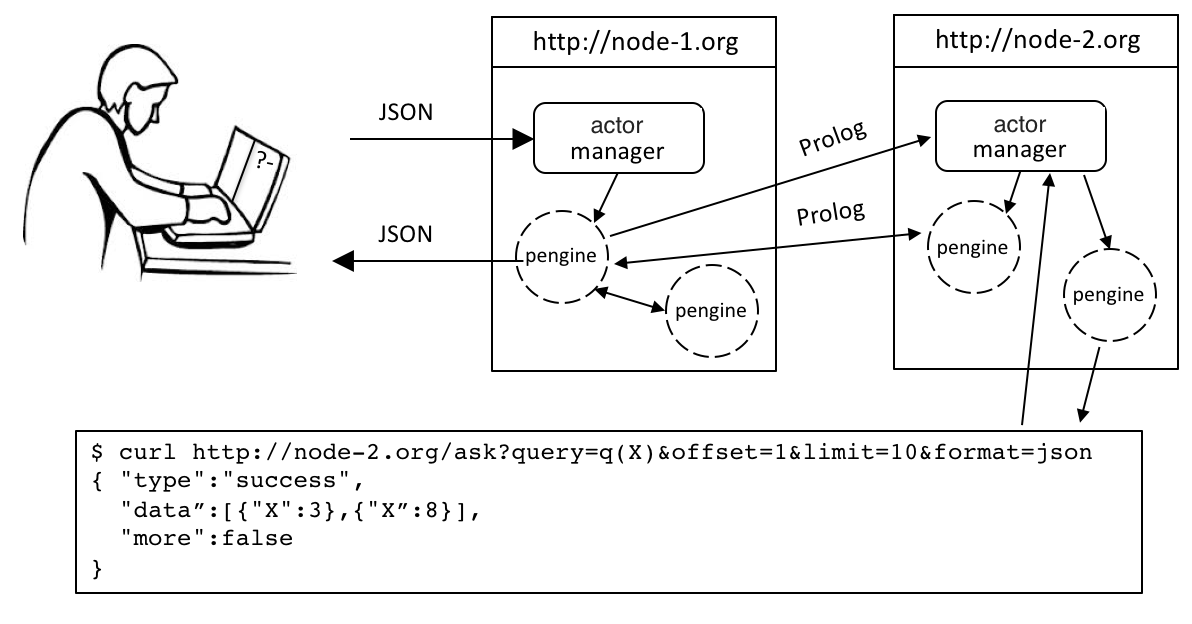
\includegraphics[width=8.2cm]{swish-pengine-interaction-2}
%    \caption{The shell offers mediated communication between a programmer and pengines populating two nodes on the Prolog Web.}
%    \label{fig:swish-pengine-interaction}
%\end{figure}

\begin{figure}[h]
    \centering
	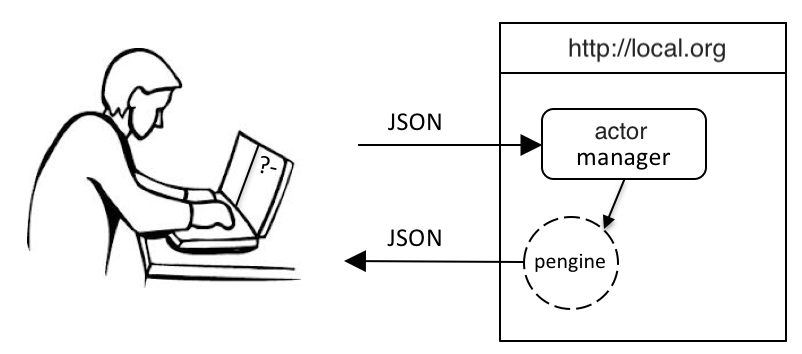
\includegraphics[width=7.3cm]{swish-pengine-interaction}
    \caption{The shell offers mediated communication between a programmer and a pengine hosted by a node.}
    \label{fig:swish-pengine-interaction}
\end{figure}

A node is an executing Web Prolog runtime environment. Its purpose is to host \textit{pengines} and other actors. A pengine is an actor and a programming abstraction modelled on the interactive top-level of Prolog. It can be seen as a first-class Prolog top-level, accessible from Web Prolog as well as from other programming languages. 

%Should the programmer decide to close or leave the IDE, the pengine with which the shell is connected will be destroyed. (As we shall see, this is related to the Erlang notion of \textit{linking}.)


\noindent Despite what Figure~\ref{fig:swish-pengine-interaction} may suggest, the programmer may not be alone in interacting with this particular node. Other programmers may be talking to other pengines running there. They are completely shielded from each other, unless the programs they are running have been written to allow them to communicate. In any case, pengines do not share memory, so in order to share information, they must exchange messages.

A node is equipped with comprehensive web APIs using WebSocket and HTTP as transport protocols, over which a client can run Web Prolog programs defined by the owner of the client, the owner of the node, or by contributions from both. The IDE must be run over the WebSocket protocol.

The task of the node's \textit{actor manager} is to handle the reception of messages sent by clients and arriving over WebSocket connections. They may be messages requesting the spawning of a pengine or termination of a pengine, or messages to be forwarded to the pengine addressed by a pid. The actor manager is also responsible for the registration and deregistration of pengines. %The registration happens right after the creation of a pengine, deregistration after it has terminated.

Crucially, a node may host a Web Prolog \textit{program} -- a deductive database, an expert system, a digital assistant, a home control system, or another kind of application -- perhaps related to AI and in need of knowledge representation and reasoning. If it does, any pengine running on the node has access to the predicates defined by this program in addition to Web Prolog built-in predicates. The program -- which we shall refer to as the \textit{node-resident} program -- is typically maintained by the owner of the node. Unless programmers are authorised to do so, they are not able to make any changes to it, only the owner is allowed to do so. However, by means of code injection in the workspace of the pengine, programmers are allowed to \textit{complement} the node-resident program with source code that they themselves have written. 

When the programmer enters the URI of the node in the browser's address field, a WebSocket connection is first established between the IDE and the node, and then used to ask the node to spawn a pengine. Messages sent to a node are strings, couched in the syntax of JSON, whereas messages arriving back from a node are expressed in either Prolog or in the JSON format. When talking to a browser, the pengine is instructed to use JSON. 

Our proof-of-concept demonstrator of a Web Prolog node is written in SWI-Prolog \cite{wielemaker:2011:tplp} and can be downloaded from \url{https://github.com/Web-Prolog}, installed and taken for a trial run. The IDE is included in the installation. The demonstrator features an interactive tutorial which provides a tour of the language. The editor and shell supports the usual interactive edit-run cycle and allow users to compose and run their own programs.\footnote{In the future, we intend to use a Web Prolog node as a back-end to SWISH \cite{DBLP:journals/corr/abs-1808-08042}, a much more mature online IDE for Prolog than the one offered by our demonstrator. See \url{https://swish.swi-prolog.org}.}


%The interaction between the shell and the pengine to which the shell is attached uses the \textit{Pengine Communication Protocol} (PCP), implemented as a WebSocket sub-protocol. The protocol will be described in Section~\ref{sec:beyond-erlang}. 

%When the programmer entered the query \texttt{?-mortal(X)}, the shell process sent a message to the node, which forwarded it to the pengine:
%
%\begin{lstlisting}
%connection.send(JSON.stringify({
%  command: 'pengine_ask',
%  pid: pid,
%  query: 'mortal(X)'
%}));
%\end{lstlisting}
%
%\noindent The shell received the following response in return:
%
%\begin{lstlisting}
%{ "type":"success",
%  "pid":"9a343810@http://local.org",
%  "data":[{"X":"socrates"}],
%  "more":true
%}
%\end{lstlisting}
%
%\noindent As a consequence, the shell was updated to show the following:
%
%\begin{lstlisting}
%?- mortal(X).
%X = socrates |
%\end{lstlisting}
%
%\noindent Since the value \texttt{true} of the \texttt{more} property of the JSON message indicated that other solutions to the query existed, a blinking cursor prompted the programmer for input, asking as it were: ``You want more, or not?''. When the programmer responded by typing a semicolon, the shell sent a \texttt{next} message to the pengine and the pengine responded with a new JSON structure representing the second solution to the query \texttt{?-mortal(X)}, and so on.
%
%Messages recognised by the shell fall under different \textit{types}. In addition to the message type that indicates success, there is a type that indicates failure of a query, and a type that indicates errors and other exceptions. Other message types are related to I/O. Would a program call \texttt{read/1} for example, the message that is sent to the shell is of type \texttt{prompt}, and when the programmer enters a term in response to the prompt, an \texttt{input} message is sent to the node and forwarded to the pengine. When the pengine calls the \texttt{writeln/1} predicate, an \texttt{output} message is sent to the shell, which knows exactly what to do with it.


\section{Erlang-Style Programming in Web Prolog}\label{sec:language}

\vspace{1mm}

\begin{quote}
Reading the code was fun -- I had to do a double take -- was I reading Erlang or Prolog -- they often look pretty much the same. \flushright \textit{Joe Armstrong} (p.c. June 18, 2018)
\end{quote}

\vspace{2mm}

\noindent Most Erlangers are probably aware that Erlang is related to Prolog in more than one way. The first implementation was written in Prolog \cite{DBLP:conf/hopl/Armstrong07}, and syntactically they look rather similar and share a lot of terminology. This is something we try to take advantage of when designing Web Prolog and we even name the predicates which support spawning and messaging after Erlang primitives with similar syntax and semantics. However, as we shall see, the primitives for spawning and messaging in Web Prolog are in some ways more expressive than the corresponding Erlang primitives.

%As we shall see, we are able to build the Prolog Web on top of them in a principled way.



\subsection{A Simple Count Server}\label{sec:count-server}

Just like in Erlang, source code which specifies the behaviour of an actor to be spawned can be written in Web Prolog -- the kind of messages it will listen for, and the kind of messages it will send to other actors. Such actors are referred to as \textit{servers} in the Erlang community.

In the editor, a count server can be written as follows and then be loaded by means of injection into the workspace of the pengine to which the shell is attached: 

\begin{lstlisting}
count_server(Count0) :-                 
    receive({             
        count(Pid) ->
            Count is Count0 + 1,    
            Pid ! Count,   
            count_server(Count);
        stop(Pid) ->
            Pid ! stopped(Pid)     
    }).                   
	                      
\end{lstlisting}

\noindent This code contains two primitives foreign to traditional Prolog. The predicate \texttt{receive/1} is used to select and extract messages appearing in the mailbox of the process running the code. The send operator \texttt{!/2} is used to send a message to another process.

The example demonstrates a programming pattern frequently found in Erlang programs and destined to become very useful in Web Prolog as well: a loop is defined where a call to the receive primitive is used to match a message in the mailbox, do something with it, and then continue looping by making a recursive call. The state of the counter is kept in the argument of \texttt{count\_server/1}.

The predicate \texttt{spawn/2-3} is used to create actor processes and it works almost like the spawn function in Erlang. However, while Erlang is a higher-order language in which the spawn function takes an anonymous function as its argument, Prolog (or Web Prolog) is not a higher-order language in this sense. In Web Prolog, \texttt{spawn/1-3} is a \textit{meta predicate} which expects a callable goal to be passed in the first argument. Also, while the spawn function in Erlang exists in more than a dozen variants, Web Prolog has only two, one which takes a list of options and one which relies on their default values. The options are used for the configuration of the actor to be created. Here is how we can spawn the count server from the shell and take it for a trial run:

\begin{lstlisting}
?- spawn(count_server(0), Pid, [
       monitor(true),
       src_predicates([count_server/1])
   ]).
Pid = '8915b2d4'.
?- self(Self).
Self = 'f431a324'@'http://local.org'.
?- $Pid ! count($Self),
   receive({Count -> true}).
Count = 1.
?- $Pid ! stop($Self).
true.
?- flush.
Shell got stopped('8915b2d4')
Shell got down('8915b2d4',true)
true.
?-
\end{lstlisting}

\noindent The \texttt{src\_predicates} option ensured that the count server source code injected into the workspace of the top-level pengine was also injected into the workspace of the spawned server process. Calling \texttt{self/1} determined the identity of the top-level pengine, and \texttt{!/2} was used to send the current count back to the client. Calling the utility predicate \texttt{flush/0} -- also borrowed from Erlang -- allowed us to inspect the content of the top-level mailbox, where a message \texttt{stopped} as well as a \texttt{down} message was found. 

Note also the use of another shell utility feature, borrowed from SWI-Prolog, which allows bindings resulting from the successful execution of a top-level goal to be reused in future top-level goals as \texttt{\$Var}. Together with \texttt{flush/0}, this facility comes in handy during interactive programming in the shell.

In addition to the \texttt{src\_predicates} option, \texttt{spawn/2-3} supports a number of other options, some of which provide alternative ways to inject source code into the workspace of an actor. Furthermore, the \texttt{node} option allows the programmer to spawn an actor process on a remote node instead of locally, and other options allow the caller to monitor the spawned process or to terminate it should the caller die.

%The count server running on the node is a child of the pengine running on the same node, which in turn is a child of the JavaScript process running the shell. This brings us to the notion of \textit{links}. 
\textit{Links} in Web Prolog are somewhat simpler than in Erlang. In contrast to Erlang's bi-directional links, they are uni-directional. As argued in \cite{conf/erlang/SvenssonFE10}, uni-directional links simplify things and do not harm expressivity. The only kind of link currently supported in Web Prolog is specified by means of an option \texttt{link} to \texttt{spawn/3} which, if set to \texttt{true} (default), causes the child process to terminate if its parent does. Only authorised clients can set it to \texttt{false} and thus an unauthorised client cannot spawn a process which is \textit{not} linked to the process that spawned it. This is to avoid leaving orphaned processes around on a node.

An obvious example of the use of links is that when a programmer closes (or just leaves) the IDE, the top-level pengine which serves the shell as well as any actors that may have been spawned from this pengine are forced to terminate. This might be seen as a supervision hierarchy rooted in the process running the shell.


\subsection{Node-Resident Actor Processes}

In addition to node-resident source code, the owner of a node may install \textit{node-resident actor processes}. We show an example below which uses \texttt{register/2} to give a running count server a mnemonic name:

\begin{lstlisting}
?- spawn(count_server(0), Pid),
   register(counter, Pid). 
\end{lstlisting}   

\noindent Just like in Erlang, the registered name can be used instead of the pid when sending to the process:

\begin{lstlisting}
?- self(Self).
Self = '51f40b45'@'http://local.org'.
?- counter ! count($Self),
   receive({Count -> true}).
Count = 1.
?- counter ! count($Self),
   receive({Count -> true}).
Count = 3.
?-
\end{lstlisting}   

\noindent Contrary to a server injected and spawned by a client, a node-resident server is accessible from any client to the node that knows the registered name of the server. (This explains why \texttt{3} rather than \texttt{2} was received in the example -- another client happened to increment the counter.)


\subsection{The Syntax of Send and Receive}

The syntax of Web Prolog is ordinary Prolog except that three infix operators (\texttt{!/2}, \texttt{when/2} and \texttt{@/2}) have been declared using \texttt{op/3}, which is the predicate for specifying user-defined operators in Prolog. 

As shown in the previous section, an actor process uses the receive primitive to extract messages from its mailbox. In Web Prolog, just like in Erlang, this operation specifies an ordered sequence of \textit{receive clauses} delimited by semicolons. A receive clause always has a \textit{pattern} (a term) and a \textit{body} of Prolog goals. Optionally, it may also have a \textit{guard}, which is a query prefixed with the \texttt{when} operator. As in Erlang, its role is to make pattern matching more expressive.

To demonstrate the use of the \texttt{when} operator and the use of two \texttt{receive/2} options that causes a goal to run on timeout, we show a priority queue example borrowed from Fred H\'ebert's textbook on Erlang \cite{Hebert:2013:LYE:2543986}. The purpose is to build a list of messages with those with a priority above 10 coming first:

\begin{lstlisting}
important(Messages) :-
    receive({
        Priority-Message when Priority > 10 ->
            Messages = [Message|MoreMessages],
            important(MoreMessages)
    },[ timeout(0),
        on_timeout(normal(Messages))
    ]).

normal(Messages) :-
    receive({
        _-Message ->
            Messages = [Message|MoreMessages],
            normal(MoreMessages)
    },[ timeout(0),
        on_timeout(Messages=[])
    ]).
\end{lstlisting}

\noindent Below, we test this program by first sending four messages to the top-level process, and then calling \texttt{important/1}:

\begin{lstlisting}
?- self(S),
   S ! 15-high, S ! 7-low, S ! 1-low, S ! 17-high.
S = 'b0f80b2d'@'http://local.org'.
?- important(Messages).
Messages = [high,high,low,low].
?- 
\end{lstlisting}

\noindent For comparison, here is H\'ebert's version of \texttt{important/0}:

\begin{lstlisting}
important() ->
    receive
        {Priority, Message} when Priority > 10 ->
            [Message | important()]
    after 0 ->
        normal()
    end.
\end{lstlisting}

\noindent Compared to the Web Prolog predicate, the Erlang function is more succinct. There are three reasons for this. First, Web Prolog has a relational syntax which does not allow nesting of calls while Erlang is a functional language where such nesting is the norm. 

Secondly, while \texttt{op/3} allowed us to define the infix \texttt{when} operator, not much can be done about the more complex \texttt{receive...after...end} construct. Instead, Web Prolog defines a binary predicate expecting an ordered sequence of receive clauses wrapped in curly brackets in its first argument and the \texttt{after...} part as a list of options specifying the behaviour around time-outs in the second argument.

Thirdly, while we could have taken advantage of the fact that an Erlang tuple such as \texttt{\{Priority,Message\}} is valid syntax in Prolog too, where it is a somewhat more complex compound term of the form \texttt{\{\}((Priority,Message))}, we chose not to. In Prolog it is always better to use less complex terms, taking up less memory. The ``pair operator'' (\texttt{-}) was a sensible choice here, but any valid Prolog term would do. %can be used in a pattern.

Three fairly major syntactic differences in such a small program -- where at least the first two contribute to the program looking neater in Erlang than in Web Prolog -- may seem like a lot for a language that tries to appear as similar as possible to Erlang. However, note that the example was chosen exactly because it highlights many differences in a tiny program. Usually, the differences are less conspicuous.

All in all, we believe that most Erlangers will find the syntax of Web Prolog likeable and easy to work with. Fans of Elixir may be less enthusiastic, at least if the Prolog-ish syntax that Erlang inherited from Prolog is what drew them to Elixir with its Ruby-ish syntax instead. %(Of course, other factors such as tooling may have been at play here as well.)


\subsection{The Semantics of Send and Receive}

Getting the semantics of \texttt{receive/1-2} right is of course more important than getting its syntax right and we believe we have succeeded in doing that. As in Erlang, \texttt{receive/1-2} scans the mailbox looking for the first message (i.e. the oldest) that matches a pattern in any of the receive clauses and satisfies the corresponding guard (if any), blocking if no such message is found. If a matching clause is found, the message is removed from the mailbox and the body of the clause is called. In Web Prolog, just like in Erlang, values of any variables bound by the matching of the pattern with a message are available in the body of the clause.

If no pattern matches a message in the mailbox, the message is \textit{deferred}, possibly to be handled later in the control flow of the process. The receive is still running, waiting for more messages to arrive, and for one that will match. Just like in Erlang, this behaviour is particularly useful if we expect two messages but are not sure which one will arrive first. Note that the implementation of the priority-queue example relies on this behaviour and would not work without it.

Most uses of receive in Erlang can be mechanically translated into uses of receive in Web Prolog that will behave in the same way as in Erlang. However, three differences should be noted. First, Erlang's receive construct is an \textit{expression} (with a value given by the expression on the right hand side of the arrow of a matching rule) rather than a statement (that will succeed or fail as in Prolog, and will not return a value). 

Secondly, Erlang enforces purity and efficiency by only allowing a restricted set of primitives in guards, and completely disallows calling user-defined functions. For the use cases the people behind Erlang had, it probably made sense to impose such restrictions. In Web Prolog, although only the first solution will be searched for, any query may be used as a guard and values of variables bound by it are available in the body. This makes the receive construct more powerful than in Erlang, but it also means that the programmer is made responsible for keeping guards as simple and efficient as possible and to avoid side effects. Enabling the programmer to condition the matching of a receive clause on the content of the whole Prolog database makes it worth it.

Finally, the receive construct in Web Prolog is a \textit{semi-deterministic} predicate, i.e. it either fails, or succeeds exactly once. As will be shown in Section~\ref{sec:beyond-erlang}, this is a key property of \texttt{receive/1-2} which ensures that backtracking can be handled in an elegant way.


\subsection{Concurrent and Distributed Programming}

Since the count server in Section~\ref{sec:count-server} is running in parallel to the pengine to which the shell is attached and is talking to it using asynchronous messaging, we have already demonstrated the use of concurrency. Below, in a probably more convincing example inspired by a user's guide to Erlang,\footnote{See \url{http://erlang.org/doc/getting_started/conc_prog.html}} two processes are first created and then start sending messages to each other a specified number of times:

\begin{lstlisting}
ping(0, Pong_Pid) :-
    Pong_Pid ! finished,
    io:format('Ping finished',[]).
ping(N, Pong_Pid) :-
    self(Self),
    Pong_Pid ! ping(Self),
    receive({
        pong ->
            io:format('Ping received pong',[])
    }),
    N1 is N - 1,
    ping(N1, Pong_Pid).
    
pong :-
    receive({
        finished ->
            io:format('Pong finished',[]);
        ping(Ping_Pid) ->
            io:format('Pong received ping',[]),
            Ping_Pid ! pong,
            pong
    }).
\end{lstlisting}

\noindent When \texttt{start/0}, defined below, is called, the behaviour of this program exactly mirrors the behaviour of the original version in Erlang.

%\newpage

\begin{lstlisting}
start :-
    spawn(pong, Pong_Pid, [
        src_predicates([pong/0])
    ]),
    spawn(ping(3, Pong_Pid), _, [
        src_predicates([ping/2])
    ]).
\end{lstlisting}

\noindent Another thing that Web Prolog has in common with Erlang is that spawning and sending work also in a distributed setting. In Web Prolog we can pass the \texttt{node} option to the spawn operation to invoke a process on a remote node and subsequently communicate with it using send and receive. For example, if the option \texttt{node('http://remote.org')} is passed to any of the above calls to \texttt{spawn/3}, the game of ping-pong will be played between two nodes.

%If the definition of \texttt{start/0} is replaced with the definition below, one of the process is spawned on a remote node:
%
%\begin{lstlisting}
%start :-
%    spawn(pong, Pong_Pid, [
%        node('http://remote.org'),
%        src_predicates([pong/0])
%    ]),
%    spawn(ping(3, Pong_Pid), _, [
%        src_predicates([ping/2])
%    ]).
%\end{lstlisting}


\subsection{Programming Patterns in Erlang and Web Prolog}\label{sec:porting-erlang}

As long as languages do deterministic and sequential computation only, i.e. when neither search nor concurrency is involved, functional programming and logic programming are fairly similar in the way they work, and methods used to achieve success with one often transfer to the other. Immutable variables, pattern matching and recursion, for example, typically play important roles in both kind of languages.

%At this point, it might be a good idea to ask ourselves to what extent we can count on being able to (more or less directly) translate Erlang programs into Web Prolog programs. The examples in this paper are too small to show much, but we have translated an Erlang program solving the Dining Philosophers problem into Web Prolog. The experience with this slightly bigger program -- which uses seven concurrently running actor processes -- convinced us that such translation is indeed fairly easy to perform. 

%In a post to the \textit{erlang-programming} list, the renowned programming wizard and Prolog and Erlang specialist Richard O'Keefe writes that he ``would argue that it is precisely the `receive' construct in Erlang that makes Erlang such a joy to use''.\footnote{\url{https://groups.google.com/forum/\#!msg/erlang-programming/gjU-HCoq7dk/Mx_Af0iQ5P0J}} Based on our own experience, we concur with this assessment. 

%In another post O'Keefe states that he ``would prefer multi-threading in Prolog to look as much as possible like Erlang''.\footnote{\url{https://groups.google.com/d/msg/erlang-programming/1jdsnqZ4XfQ/ve9WfFl2YBwJ}} We agree here too, but note that it might be too late since at least four Prolog systems have already implemented the proposed ISO Prolog standard for multi-threading. For a special-purpose dialect such as Web Prolog, Erlang-style concurrency appears to be an excellent choice.

When concurrency \textit{is} involved, language designers must choose a good approach and a suitable set of primitives to express it. In a post to the \textit{erlang-programming} mail list, the renowned programming wizard and Prolog and Erlang specialist Richard O'Keefe writes that he ``would prefer multi-threading in Prolog to look as much as possible like Erlang''.\footnote{\url{https://groups.google.com/d/msg/erlang-programming/1jdsnqZ4XfQ/ve9WfFl2YBwJ}} We do agree, but note that it might be too late since at least four Prolog systems have already implemented the proposed ISO Prolog standard for multi-threading.\footnote{\url{https://logtalk.org/plstd/threads.pdf}} Be that as it may, for a special-purpose dialect such as Web Prolog, Erlang-style concurrency appears to be an excellent choice, especially since it generalises to the distributed case as well.

As a consequence of this choice, Erlang and Web Prolog share not only a great deal of syntax and a lot of terminology  but many programming patterns as well, such as the use of concurrency and recursion for maintaining state, the use of protocols, and various abstractions for asynchronous and synchronous communication between processes which may or may not run on the same machine or CPU core. Indeed, as the programs in Section~\ref{sec:language} demonstrated, it is usually straightforward to translate Erlang programs into Web Prolog. %Unnesting of functional notation, for example, is a purely syntactical operation that can be done mechanically.


%At this point, it might be a good idea to ask ourselves to what extent we can count on being able to (more or less directly) translate Erlang programs into Web Prolog programs. The examples in this paper are too small to show much, but we have translated an Erlang program solving the Dining Philosophers problem into Web Prolog. The experience with this slightly bigger program -- which uses seven concurrently running actor processes -- convinced us that such translation is indeed fairly easy to perform. 

The close affinity between Erlang and Web Prolog leads us to believe that behaviours such as those offered by the OTP might be implemented in future versions of Web Prolog. To ensure the uninterrupted service of node-resident actors, for example, the supervisor behaviour would be great to have, and as a way to implement complex protocols in the style of Erlang, the state machine behaviour might be useful.


%Below, we investigate the change of behaviour introduced by passing the \texttt{monitor} option to \texttt{spawn/3} in more detail. Here is an example:
%
%\begin{lstlisting}
%?- self(Self),
%   spawn((mortal(Who), Self ! Who), Pid, [
%       monitor(true)
%   ]).
%Pid = '88a67bd4', 
%Self = '9d03409e'@'http://local.org'.
%?-
%\end{lstlisting}
%
%\noindent In this way, we made sure the spawning process is informed about what eventually will be the fate of the spawned process. Let us use \texttt{flush/0} to find out what happened to it:
%
%\begin{lstlisting}
%?- flush.
%Shell got socrates
%Shell got down('88a67bd4'@'http://local.org',true)
%true.
%?- 
%\end{lstlisting}
%
%\noindent The second of these messages serves to inform the spawning process that the spawned process has terminated and \texttt{true} in the second argument of the message term means the goal succeeded (whereas \texttt{false} would have meant it failed). Replacing the subgoal \texttt{mortal(Who)} with (say) \texttt{happy(Who)} would (since \texttt{happy/1} is not defined) result in just one \texttt{down} message with a detailed error message in the second argument.
%
%An actor is spawned on the initiative of a client that is itself an actor or another process (e.g. a shell process). If the value of the \texttt{link} option is \texttt{true}, it means that when the client terminates the child actor also terminates. For an authenticated user with the right authorisation it will be possible to set the \texttt{link} option to \texttt{false} in order to create what we think of as an \textit{independent} and possibly (or even typically) \textit{long running} actor. Such actors are free, not dependent on their lives on their creators. 
%
%Consider the case of an anonymous JavaScript client A, spawning a process on a node B, which in turn spawns two processes C and D. These four processes form a rather simple and rigid supervisor hierarchy: if A terminates, then B terminates too, and if B terminates, then C and D also terminates. At least for anonymous clients, this is the only rule. Authenticated and authorised users may be permitted to create processes on a node that do not terminate when the parent terminates.




%Termination can be automated. As a practical example let us consider how to implement a supervisor behavior using a uni-directional link. Assuming we want to supervise a child process, specified as the goal \texttt{foo(X)}, so that if the supervisor terminates, the child terminates too, then the following supervisor code fragment suffices: 
%
%\begin{lstlisting}
%...
%spawn(foo(X), Pid, [link(true)]),
%...
%\end{lstlisting}
%
%\noindent This very rigid supervisor hierarchy can be seen as an extreme case of an approach to error handling which by Erlang programmers is often referred to as ``let it crash''. If a user starts a process that spawns other processes (and in turn yet other processes) and something goes wrong, he can usually just make a new attempt. This is an approach that should be good enough for the Web. 
%
%Erlang offers a great deal of flexibility with respect to the way the graceful termination or crash of a process influences other processes to which it is related. In Erlang, such mechanisms are programmable, not hardwired. This is true for Web Prolog as well. In Web Prolog, it is easy to get the impression that they are hard wired, but the need to impose a strict master-slave regime comes from the need to avoid leaving orphaned processes around, and is not a limitation of the language. It would be possible to allow authenticated and authorised users to spawn processes that do not terminate when the process that spawned them terminates, i.e. to allow the creation of processes that outlive its creator.


\section{Backtracking beyond Erlang}\label{sec:beyond-erlang}

As we now turn to examples that go beyond what Erlang can easily do, it is probably wise to entertain a suspicion of unexpected interactions between language features and possible impedance mismatches between the two paradigms -- between Prolog's relational, non-deterministic programming model and Erlang's functional and message passing model. How well do the Erlang-ish constructs mix with backtracking for example? In the next section we show an example which suggests that the mix is both sound and easy to understand. 

\subsection{Handling Non-determinism}\label{sec:non-det}

%In theory, we should be on the safe side. Sequential Erlang is basically Erlang with its data types, one-way pattern matching, functions and control structures, but without spawn, send, receive, and other constructs designed for concurrent programming. The idea behind Web Prolog can thus be described as an attempt to ``plug out'' the sequential part from Erlang and ``plug in" sequential Prolog instead. There seems to be no principled reasons why we would not be able to replace the sequential functional language with a sequential relational language, e.g. a logic programming language such as Prolog. Indeed, in \cite{armstrong2003concurrency} Joe Armstrong  writes:
%
%\begin{quote}
%Erlang is a concurrent programming language with a functional core. By this we mean that the most important property of the language is that it is concurrent and that secondly, the sequential part of the language is a functional programming language.
%\end{quote}
%
%\begin{quote}
%The sequential subset of the language expresses what happens from the point it time where a process receives a message to the point in time when it emits a message. From the point of view of an external observer two systems are indistinguishable if they obey the principle of observational equivalence. \textit{From this point of view, it does not matter what family of programming language is used to perform sequential computation.} (Our emphasis.)
%\end{quote}

\noindent Suppose the query given in the argument to \texttt{spawn/2} has more than one answer, a query such as \texttt{?-mortal(Who)} for example. Below, a goal containing this query is called, the first solution is sent back to the calling process, and then \texttt{receive/1} is used in order to listen for a message of the form \texttt{next} or \texttt{stop} before terminating:

\begin{lstlisting}
?- self(Self),
   spawn(( mortal(Who),
           Self ! Who,
           receive({
               next -> fail;
               stop -> true
           })
         ), Pid).
Pid = 'a4b940a8',
Self = 'c4806702'@'http://local.org'.
?- flush.
Shell got socrates
true.
?- $Pid ! next.
true.
?- flush.
Shell got plato
true.
?- $Pid ! stop.
true.
?-
\end{lstlisting}

\noindent As this session illustrates, the spawned goal generated the solution \texttt{socrates}, sent it to the mailbox of the Prolog top-level and then suspended and waited for messages arriving from the top-level process. When the message \texttt{next} arrived, the forced failure triggered backtracking which generated and sent \texttt{plato} to the mailbox of the top-level shell process. The next message was \texttt{stop}, so the spawned process terminated.

For an Erlang programmer this particular use of \texttt{receive/1} may come as a surprise. After all, the Prolog concepts of \textit{failure} and \textit{backtracking} and the use of failure to force backtracking are foreign to Erlang. Prolog programmers may recognise a behaviour due to the fact that \texttt{receive/1-2} is a \textit{semi-deterministic} predicate, i.e. a predicate that either fails, or succeeds exactly once. The only way \texttt{receive/1-2} will fail is if the goal in the \textit{body} of one of its receive clauses fails. To see how it pans out in a corner case, consider the following two receive calls:

\begin{lstlisting}
receive({m(X) -> true})     receive({m(X) -> fail})
\end{lstlisting} 

\noindent The call on the left will succeed if a message matching the pattern \texttt{m(X)} appears in the mailbox. The call on the right will fail (and possibly cause backtracking) once a message matching the pattern \texttt{m(X)} appears. Only by the left call will the variable \texttt{X} be bound. Both calls will remove the matched message from the mailbox.

The tiny examples in this section highlighted a vital feature of the Web Prolog design as they showed how Prolog-style search and Erlang-style concurrency can be integrated and how a non-deterministic query can be supplied with a deterministic interface. This is precisely the point where the logic programming model and the actor programming model -- represented here by Prolog and Erlang -- interface with each other. This suggests that Prolog's backtracking mechanism is perfectly compatible with, and in fact complements, the proposed Erlang-like mechanisms for spawning actors and handling the communication between them.

The first example above demonstrated an actor adhering to what might be seen as a tiny communication protocol accepting only the messages \texttt{next} and \texttt{stop}. We need to observe, however, that the goal to be solved was hard-coded into the program, and that the program handles neither failure of the spawned goal, nor exceptions thrown by it. There is clearly a need for something more generic. In the next section we will describe the API to a full-blown generic pengine abstraction -- an actor adhering to a considerably more complex protocol.


\subsection{A Pengine is an Actor with a Protocol}

In traditional Prolog the top-level is \textit{lazy} in the sense that new solutions to a query are only computed on demand. However, the top-level is not accessible to programs, i.e. a program cannot \emph{internally} create a top-level, pose queries and request solutions on demand. In Web Prolog, a pengine is a programming abstraction modelled on the interactive top-level of Prolog. A pengine is like a first-class interactive Prolog top-level, accessible from Web Prolog as well as from other programming languages such as JavaScript. 

%We refer to a pengine as an \textit{encapsulated Prolog session}, an abstraction designed to make Prolog programmers feel right at home.

What distinguishes a pengine from other kinds of actors is the \textit{protocol} it follows when it communicates, i.e. the kind of messages it listens for, the kind of messages it sends, and the behaviour this gives rise to. The protocol must not only allow a client to ask queries and a pengine running on a node to respond with answers, it must also allow the pengine to prompt for input or produce output in an order and with a content as dictated by the running Web Prolog program. All pengines follow this protocol. The shell adheres to it as well, and even a human user of a shell talking to a pengine must adapt to it in order to have a successful interaction with the pengine.

The design behind pengines is in fact inspired by the informal communication protocol that we as programmers adhere to when we invoke a Prolog shell from our OS prompt, load a program, submit a query, are presented with a solution (or a failure or an error), type a semicolon in order to ask for more solutions, or hit return to stop. These are ``conversational moves'' that Prolog understands. There are even more such moves, since after having run one query to completion, the programmer can choose to submit another one, and so on. The session does not end until the programmer decides to terminate it. There are only a few moves a client can successfully make when the protocol is in a particular state, and the possibilities can easily be described, by a state machine for example, as we shall do in the next section.



\subsection{The Pengine Communication Protocol}\label{sec:pcp}

%As is often pointed out by Joe Armstrong, message-based systems give us a whole new level of abstraction. In his words, ``We have the black boxes that do things, and we have the messages in between. What goes on inside the black boxes does not really matter; what takes place there is abstracted over.'' This is just as true for pengines and multi-pengine systems as it is for other actors and actor systems. As long as a process delivers correct answers in response to Prolog queries over a Prolog program, it can, for all intents and purposes, be counted as a pengine.

Figure~\ref{fig:statechart} depicts a statechart specifying the Pengine Communication Protocol (PCP) -- a protocol for the communication between a client and a server (in the Erlang sense of these terms). The server is a pengine running on a node. The client can be any process (including another actor or a JavaScript process) capable of sending the messages and signals in bold to the server. The server is responsible for returning the messages with a leading / back to the client.\footnote{The use of a statechart allows us to show that no matter the current state of the protocol, \textbf{abort} will always take it to the state from which a new query can be asked and \textbf{exit} will always terminate the pengine process.}



%Suppose, for example, that the current state of the protocol is \textbf{s2}, and that the \textbf{abort} signal is received. The transitions leaving \textbf{s2} are tried from the inside and out, and since no label on a transition leaving \textbf{s2} matches, but one placed one step higher in the hierarchy does, a transition to state \textbf{s1} takes place.

\begin{figure}[h]
    \centering
	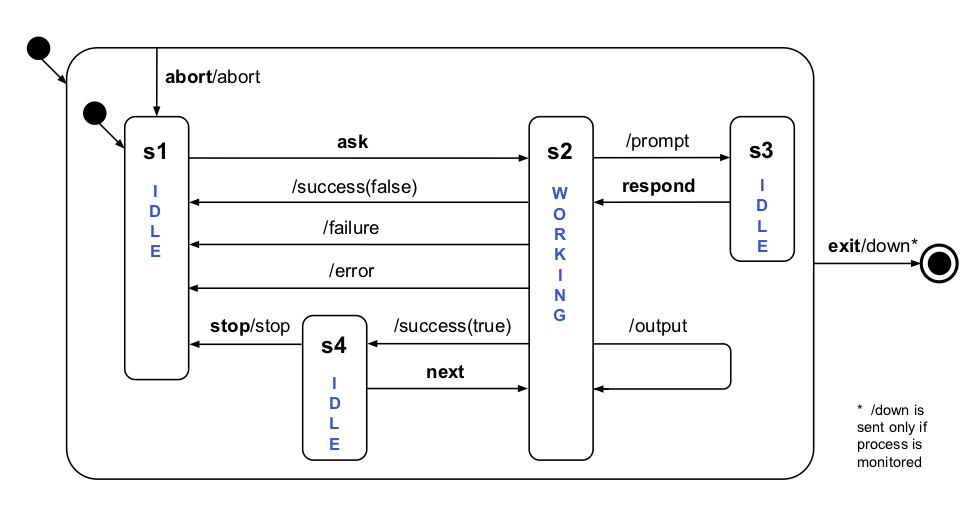
\includegraphics[width=8.5cm]{statechart}
    \caption{Statechart specifying the PCP for a complete Web Prolog session. The transitions are labeled with \textit{message types}. Types in bold are sent from the client to the pengine, whereas message types with a leading / goes in the opposite direction, from the pengine to the client.}
    \label{fig:statechart}
\end{figure}

\noindent Web Prolog comes with built-in predicates which allow a client to spawn a pengine (\texttt{pengine\_spawn/1-2}), and send it messages in bold (\texttt{pengine\_ask/2-3}, \texttt{pengine\_next/1-2}, \texttt{pengine\_stop/1}, \texttt{pengine\_respond/2}, \texttt{pengine\_abort/1} and \texttt{pengine\_exit/1}). For communication from the pengine to the client, \texttt{pengine\_input/2} and \texttt{pengine\_output/1} are available.


\subsection{In Conversation with a Pengine}

Below, we show how to create and interact with a pengine process that runs as a child of the current top-level process. %Indeed, what we have here is a pengine running another pengine, a Prolog top-level running another Prolog top-level:

\begin{lstlisting}
?- pengine_spawn(Pid, [
       node('http://remote.org'),
       src_text("p(a). p(b). p(c)."),
       monitor(true),
       exit(false)
   ]),
   pengine_ask(Pid, p(X), [
       template(X)
   ]).
Pid = '7528c178'@'http://remote.org'.
?- flush.
Shell got success('7528c178'@'http://...',[a],true)
true.
?- pengine_next($Pid, [
       limit(2)
   ]),
   receive({Answer -> true}).
Answer = success('7528c178'@'http://...',[b,c],false).
?-
\end{lstlisting}

\noindent There is quite a lot going on here. The \texttt{node} option passed to \texttt{pengine\_spawn/1-2} allowed us to spawn the pengine on a remote node, the \texttt{src\_text} option was used to send along three clauses to be injected into the process, and the \texttt{monitor} options allowed us to monitor it. These options are all inherited from \texttt{spawn/2-3}.

Given the pid returned when calling \texttt{pengine\_spawn/1-2}, we then called \texttt{pengine\_ask/2-3} with the query \texttt{?-p(X)}, and by passing the \texttt{template} option we decided the form of answers. Answers were returned to the mailbox of the calling process (i.e. in this case the mailbox belonging to the pengine running our top-level). We inspected them by calling \texttt{flush/0}. By calling \texttt{pengine\_next/2} with the \texttt{limit} option set to \texttt{2} we then asked for the last two solutions, and this time used \texttt{receive/1} to view them.

We passed the option \texttt{exit(false)} to \texttt{pengine\_spawn/2}, so although the query has now run to completion, the pengine is not dead and we can use it to demonstrate how I/O works:

\begin{lstlisting}
?- pengine_ask($Pid, pengine_output(hello)),
   receive({Answer -> true}).
Answer = output('7528c178'@'http://remote.org',hello).
?-
\end{lstlisting}

\noindent We will not show it here, but input can be collected by calling \texttt{pengine\_input/2}, which sends a \texttt{prompt} message to the client which can respond by calling \texttt{pengine\_respond/2}. 

\noindent The pengine is still not dead so let us see what happens when a non-terminating query such as \texttt{?-repeat,fail} is asked:

\begin{lstlisting}
?- pengine_ask($Pid, (repeat, fail)).
true.
?-
\end{lstlisting}

\noindent Although nothing is shown, we can assume that the remote pengine is just wasting CPU cycles to no avail. Fortunately, we can always abort a runaway process by calling \texttt{pengine\_abort/1}:

\begin{lstlisting}
?- pengine_abort($Pid),
   receive({Answer -> true}).
Answer = abort('7528c178'@'http://remote.org').
?-
\end{lstlisting}

\noindent When we are done talking to the pengine we can kill it:

\begin{lstlisting}
?- pengine_exit($Pid, goodbye),
   receive({Answer -> true}).
Answer = down('7528c178'@'http://remote.org',goodbye).
?-
\end{lstlisting}

\noindent Note that messages sent to a pengine will always be handled in the right order even if they arrive in the ``wrong'' order (e.g. \texttt{next} before \texttt{ask}). This is due to the selective receive which defers the handling of them until the PCP protocol permits it. This behaviour guarantees that pengines can be freely ``mixed'' with other pengines or actors. The messages \texttt{abort} and \texttt{exit}, however, will never be deferred.

\subsection{Non-deterministic RPC}\label{sec:ndrpc} 

For the purpose of a very straightforward approach to the distribution of programs over two or more nodes, Web Prolog offers \texttt{rpc/2-3}, a meta-predicate for making non-deterministic remote procedure calls. Such calls are synchronous and no explicit concurrency is involved, and this is what makes \texttt{rpc/2-3} remarkably easy to use.

The \texttt{rpc/2-3} predicate allows a process running in a node A to call and try to solve a query in the Prolog context of another node B, taking advantage of the data and programs being offered by B, just as if they were local to A. (Recall that \texttt{pengine\_spawn/1-2} can also do this, but only in a more roundabout way.) A Web Prolog client process queries a node by calling \texttt{rpc/2} with the first argument a URI pointing to the node, and the second argument a query to be run over the predicates offered by the node. Here is a trivial example of its use:

\begin{lstlisting}
?- rpc('http://remote.org', mortal(Who)).
Who = socrates ;
Who = plato ;
Who = diogenes.
?-
\end{lstlisting}

%\noindent Interestingly, \texttt{rpc/2-3} retains the logical purity of the predicates it calls, i.e. if the query that is called in the second argument is pure, then the entire call is pure.\footnote{This is a property it shares with the \texttt{call/N} family of Prolog predicates.}

\subsection{An Implementation of rpc/2-3}\label{sec:rpc-implementation}

Below, we show an implementation of \texttt{rpc/2-3} which is built on top of a pengine spawned on a remote node and a local loop that waits for answers arriving from it:

%This section looks at an implementation of \texttt{rpc/2-3} with code clean enough to nail down its semantics. The implementation is built on top of a pengine spawned on a remote node and a local loop that waits for answers. %From this point on the communication is synchronous:

\begin{lstlisting}
rpc(URI, Query, Options) :-
    pengine_spawn(Pid, [
         node(URI),
         exit(true),
         monitor(false)
       | Options
    ]),
    pengine_ask(Pid, Query, Options),
    wait_answer(Query, Pid).
\end{lstlisting}

\begin{lstlisting}
wait_answer(Query, Pid) :-
    receive({
        failure(Pid) -> fail;            
        error(Pid, Exception) -> 
            throw(Exception);                  
        success(Pid, Solutions, true) -> 
            (   member(Query, Solutions)
            ;   pengine_next(Pid), 
                wait_answer(Query, Pid)
            );
        success(Pid, Solutions, false) -> 
            member(Query, Solutions)
    }).
\end{lstlisting}

\noindent Note how the disjunction in the body of the third receive clause and the use of \texttt{member/2} in the third and fourth clauses turn the deterministic calls made by \texttt{pengine\_ask/3} and \texttt{pengine\_next/1} into the expected non-deterministic behaviour of \texttt{rpc/2-3}. 

%It may be helpful to think of what is going on here as a very simple kind of \textit{buffering}, and in particlar as the use of what is usually referred to as a \textit{bounded buffer}. The value of the \texttt{limit} option represents the size of the buffer. The producer (i.e. the remote pengine process) is allowed to get ahead of the consumer (i.e. the process running the \texttt{rpc/3} call), but only until the buffer is full. The consumer can take elements from the buffer immediately without waiting. When the buffer is empty, the producer is prompted to produce more elements, until the buffer is full. In our proof-of-concept implementation, the consumer and the producer are not running concurrently (as they do not execute different tasks during overlapping periods of time). A possible optimisation would be to allow them to do so by letting the remote process compute additional solutions while waiting for a \texttt{next} message and return all available solutions if it arrives. If a \texttt{stop} message arrives instead, or if time has run out, the additional solutions would be discarded. Note that nothing here concerns the client, as it is the owner of the node who would need to enable this optimisation.

%This implementation is clean enough to nail down the semantics of \texttt{rpc/2-3}, but it only works over a WebSocket connection. However, it turns out that a version of \texttt{rpc/2-3} with the exact same semantics can instead be implemented on top of the stateless HTTP described in Section~\ref{sec:browser}. This implementation is more complex, so we do not show it here.

\subsection{Reducing the Number of Network Roundtrips}\label{sec:reducing-roundtrips}

Time spent in remote shell-pengine or pengine-pengine interaction can be the dominant factor in the user-perceived performance of a web application. Some of the backtracking involved in the search for solutions is taking place over the network, and network roundtrips take time -- a lot of time in comparison with other computational steps programs typically perform. Since calling a remote program may involve very many roundtrips during backtracking, the times may add up to a significant slowdown compared to making a local call. By passing the \texttt{limit} option to \texttt{rpc/3} (inherited from \texttt{pengine\_ask/3}) we can make the communication less ``chatty'' and avoid many roundtrips. Here is an example:

\begin{lstlisting}
?- rpc('http://remote.org', mortal(Who),[
       limit(10)
   ]).
Who = socrates ;
Who = plato ;
Who = diogenes.
?-
\end{lstlisting}

\noindent As the example tries to convey, the behaviour of the call, as seen from the point of view of the client, does not change. After having been presented with the first solution to the query the programmer still needs to type a semicolon in order to see the next solution. But under the hood, the next solution has already been computed and returned to the client as the second member of a list containing all three solutions. Thus no new request to the node needs to be made. So while the retrieval of the three solutions to the query required three network roundtrips before we applied the option, it will now only require one roundtrip. More generally, a query with $n$ solutions would (normally and by default) require $n$ roundtrips if we wanted to see them all, but if we set \texttt{limit} to $i$, the same query would only require $n/i$ roundtrips, or just one roundtrip if $n/i < 1$.

Use of the \texttt{limit} option is fine also from a purity point of view -- it has nothing to do with logic and the declarative reading of the query, but must be treated as a \textit{pragma} -- as a language construct that specifies the granularity with which the conversation between the client and the node should be conducted. Passing the option \texttt{limit(10)} can be understood as saying: ``Send me the answers in chunks of \texttt{10}. I will be looking at them one-by-one, but I want them in batches.'' Although adding the limit pragma to a query will have no effect on the meaning of the query, it can have a significant effect on performance when running the query over a cluster of nodes.


\subsection{Shuffling Code and Data Back and Forth}

On the internet, the cost of shuffling code and data back and forth across remote boundaries is significant, yet cannot be avoided. But in which direction should the shuffling be made in order to bring down the cost? The answer is most likely that it varies and that programmers should be given a choice.

%It is often more efficient to bring a few lines of code to the data rather than moving an often large amount of data to the code. In the case of data being frequently updated (think stock market data for example) the gain is probably significant. On the other hand, if the data is more or less static (think geo-political data for example) and we want to query it a lot, then bringing the data to the code may be more efficient.

The obvious way to bring code to the data in Web Prolog is to inject source code into the remote process created by \texttt{rpc/2-3}. With the following call, we do just that:

\begin{lstlisting}
rpc('http://remote.org', foo(X), [
    src_text("foo(X) :- mortal(X).")
])
\end{lstlisting}

\noindent The default value of the \texttt{node} option for \texttt{spawn/2-3} and \texttt{pengine\_spawn/1-2} is the special-purpose URI \texttt{localnode}. Thus it follows, perhaps a bit counter-intuitively, that in combination with the \texttt{src\_uri} option \texttt{rpc/3} can also be used to bring the data to the code. Here is an example:


\begin{lstlisting}
rpc(localnode, mortal(X), [
    src_uri('http://remote.org/src')
])
\end{lstlisting}

\noindent The source held by the node at \texttt{http://remote.org} is injected into the workspace of the underlying pengine before the query \texttt{?-mortal(X)} is tried, thus isolation is provided.

These two examples suggest a useful symmetry which allows Web Prolog code to flow in either direction, from the client to the node or from the node to the client. The choice is determined by the programmer's selection of options configuring the actor to be spawned, but it can in principle also be decided programmatically at runtime.

%When discussing the bringing of ``code to the data'' versus ``data to the code'', it is important to keep in mind that the distinction between code and data is not as sharp in Prolog as it is in most other programming languages.

\vspace{-2mm}

\subsection{More about the Underlying Web APIs}

An IDE for traditional Prolog is a fairly demanding type of web application. Although the conversation between the programmer and the pengine must always be initiated by the programmer using the shell, the interaction may at any point turn into a mixed-initiative conversation driven by requests for input made by a running query. What makes unconstrained mixed-initiative interaction feasible is the support for efficient bi-directional messaging offered by a node thanks to the use of the WebSocket protocol.

Other kinds of web applications may have no need for mixed-initiative interaction. In order to serve such applications, a Web Prolog node offers a stateless HTTP API. Interestingly, it also turns out that since \texttt{rpc/2-3} does not produce output or request input, it can be run over HTTP instead of over the WebSocket protocol. In our proof-of-concept implementation this is the default transport.


% in addition to the stateful WebSocket API.

To retrieve the first solution to \texttt{?-mortal(X)} using HTTP, a GET request can be made with the following URI:

\vspace{-1mm}
\begin{lstlisting}
http://remote.org/ask?query=mortal(X)&offset=0 
\end{lstlisting}

\vspace{-1mm}
\noindent Here too, responses are returned as Prolog or as Prolog variable bindings encoded as JSON. Such URIs are simple, they are meaningful, they are declarative, they can be bookmarked, and responses are cachable by intermediates. 

To ask for the second and third solution to \texttt{?-mortal(X)}, another GET request can be made with the same query, but setting \texttt{offset} to \texttt{1} this time and adding a parameter \texttt{limit=2}. In order to avoid recomputation of previous solutions, the actor manager keeps a pool of active pengines. For example, when the actor manager received the first request it spawned a pengine which found and returned the solution to the client. This pengine -- still running -- was then stored in the pool where it was indexed on the combination of the query and an integer indicating the number of solutions produced so far (i.e. \texttt{1} in this case). When a request for the second and third solution arrived, the actor manager picked a matching pooled pengine, used it to compute the solutions, and returned them to the client. Note that the second request could have come from any client, not necessarily from the one that requested the first solution. This is what makes the HTTP API stateless.

The maximum size of the pool is determined by the node's settings. To ensure that the load on the node is kept within limits, the oldest active pengines are terminated and removed from the pool when the maximum size is reached. This \textit{may} mean that some solutions to some subsequent calls must be disposed of, but this will not hurt the general performance.


\section{Previous Work}\label{sec:previous}

Technology-wise, Web Prolog can be seen as an attempt to rethink and redesign our work on \texttt{library(pengines)} \cite{DBLP:journals/tplp/LagerW14}, which is the library serving SWISH \cite{DBLP:journals/corr/abs-1808-08042}. As a library for JavaScript-Prolog communication it works well enough to support SWISH, but it also makes promises that it cannot really live up to, in particular when it comes to concurrent and distributed programming. It is not possible, for example, to spawn two remote pengines and make them play ping-pong with each other. One way to put it is to say that \texttt{library(pengines)} fails to implement the actor model. %or perhaps, that it is an incomplete implementation of this model. 
A layer of predicates beneath the pengine abstraction in the form of a small set of programming primitives that support actor-based programming is a much better design, and in addition establishes a clear and direct link to Erlang.

\vspace{-0.05cm}


\section{Discussion}\label{sec:discussion}

\begin{quote}
Communicating Prolog engines is a great idea -- this is more or less what Erlang started as -- but I didn't like the idea of backtracking over nodes. \flushright \textit{Joe Armstrong} (p.c. June 16, 2018)
\end{quote}

\vspace{2mm}

\noindent The ability to backtrack over nodes must indeed be seen as part of the essence of Web Prolog. Basing the distribution of Prolog processes on the actor programming model seems to require this ability. If the idea of backtracking over nodes is abandoned, then the idea of backtracking \textit{within} an actor or over actors \textit{within} a node does not seem attractive either. Thus, the move to a functional language with its simpler syntax and deterministic operational semantics becomes the logical next step -- a step that unfortunately, as it were, does away with the ``logic'' in ``logic programming'' and with a lot of useful features that a language such as Prolog provides.

We hasten to add that in no way should this be seen to imply that we think that Armstrong and the other inventors of Erlang made a \emph{mistake} when they abandoned Prolog in favour of a simple functional language. Given that Prolog is fairly difficult to learn and to use correctly, given the nature of the problems with programming telephone switches that they set out to solve, and perhaps in an attempt to avoid being dragged down by the post fifth generation dismissal of logic programming, they probably made the right decision. After all, Erlang is a very successful programming language, more successful than Prolog when it comes to industrial uses.

Almost fifty years have gone by since Prolog was introduced as a promising language for AI, and more than thirty years have passed since Erlang was invented. Today, AI is booming again, Prolog has evolved considerably, the internet is much faster and a lot more reliable than it used to be, the multi-core hardware revolution is in full swing, and Erlang-style concurrency has emerged as a sensible way to program such hardware. Perhaps now is the right time for the idea of communicating Prolog processes and backtracking over nodes to make a comeback. With this paper we are making an attempt to show how this idea might be realised.

\vspace{-1mm}
\subsection{A Hierarchy of Useful Abstractions}\label{sec:hierarchy-of-abstraction}

In Web Prolog, just like in Erlang, the actor is regarded as the fundamental unit of computation and as the single abstraction that solves the two problems of concurrency and distribution and provides a form of network transparency. In Web Prolog, just like in Erlang, other network-transparent programming abstractions can be built on top of the actor. In Web Prolog, the most prominent and universally useful such abstraction is the pengine, followed closely by the abstraction for making non-deterministic remote procedure calls. These are both abstractions that would not fit easily into Erlang, but which are natural in Web Prolog. Abstractions such as these can be compared to Erlang \textit{behaviours}. They are not always easy to build, but once they are built they can easily be instantiated and tailored to specific tasks. 

We note that these three abstractions -- the actor, the pengine and the remote procedure call -- form a hierarchy where predicates on the higher levels inherit some of their options from predicates on the lower levels. \texttt{rpc/3} inherits options from \texttt{pengine\_spawn/2} and \texttt{pengine\_ask/3}, and \texttt{pengine\_spawn/2} inherits options from \texttt{spawn/3} in turn. 



%The node, populated by pengines and other actors, can perhaps be seen as yet another abstraction. When the stateless HTTP API is used to communicate with a node, the identities of any pengines involved are hidden.
%
%Finally, as we shall see, the Prolog Web can be seen as an abstraction as well.

\vspace{-1mm}
\subsection{Web Prolog and the Programmable Prolog Web}\label{sec:for-erlangers-2}

A node has a dual identity. It can be seen not only as a Web Prolog runtime system but also as a node in the network forming what we will refer to as \textit{the Prolog Web}. The traditional Web is distributed, decentralised and open, and these are traits we want the Prolog Web to share. Whereas distribution is nicely conceptualised in the actor model, and nicely handled by an actor programming language such as Erlang or Web Prolog, decentralisation and openness require features we choose to rely on the Web as such to contribute.

Here, the humble URI is a key concept, as it allows us to link a Web Prolog program to another Web Prolog program, a running actor to another running actor, or a Prolog query to its answers, in much the same way as HTML documents are linked to other HTML documents.

Another key feature of the Prolog Web is that communication among nodes relies only on HTTP and the WebSocket protocol. This allows it to pass through firewalls, and provides security-related features such as methods for authentication, HTTPS and CORS (Cross-Origin Request Sharing).\footnote{\url{https://en.wikipedia.org/wiki/Cross-origin_resource_sharing}}

Distributed programming in Erlang typically involves a number of nodes connected into a cluster. Erlang nodes usually rely on TCP/IP for transport and are, for reasons of security, assumed to be operating in a closed, trusted environment where we directly control the machines involved. In other words, when Erlang runs on a cluster, it is a cluster that is \textit{closed}. In comparison, the Prolog Web might be seen as a cluster as well, but one that is as \textit{open} as the Web itself. %, and just as open as the Web itself.

%In the context of Web Prolog we can compare an Erlang cluster to what we refer to as \textit{the Prolog Web}. We think of the Prolog Web as an extension of the traditional Web, but it might be seen as a cluster as well, but one that is \textit{open}. 


%\subsection{Web Prolog and the programmable Prolog Web 2}\label{sec:for-erlangers-2}
%
%Distributed programming in Erlang typically involves a number of nodes connected into a cluster. Erlang nodes usually rely on TCP/IP for transport and are, for reasons of security, assumed to be operating in a closed, trusted environment where we directly control the machines involved. In other words, when Erlang runs on a cluster, it is a cluster that is \textit{closed}.
%
%In the context of Web Prolog we can compare an Erlang cluster to what we refer to as \textit{the Prolog Web}. We think of the Prolog Web as an extension of the traditional Web, but it might be seen as a cluster as well, but one that is \textit{open}. 
%
%The traditional Web is distributed, decentralised and open and these are traits we want the Prolog Web to inherit. Whereas distribution is nicely conceptualised in the actor model, and nicely handled by an actor programming language such as Erlang or Web Prolog, decentralisation and openness require features we choose to rely on the Web as such to contribute. 
%
%Here, the humble URI is a key concept, as it allows us to link a Web Prolog program to another Web Prolog program, a running actor to another running actor, or a Prolog query to its answers, in much the same way as HTML documents are linked to other HTML documents.
%
%The Prolog Web relies only on web APIs based on HTTP and the WebSocket protocol. This allows communication to pass through firewalls, and implements various security-related features such as methods for authentication, Secure websockets (i.e. websockets over HTTPS) and CORS (Cross-Origin Request Sharing).

%\footnote{\url{https://en.wikipedia.org/wiki/Cross-origin_resource_sharing}

%\vspace{-2mm}

\subsection{Would the Prolog Web Scale?}

By adopting a computational model capable of scaling out not only to multiple cores on one machine but also to multiple nodes running on multiple machines, by introducing an option allowing clients to limit the number of network roundtrips it takes to run a query to completion, by embracing the WebSocket transport protocol with its low overhead per message, by offering also a stateless HTTP API, and by leaving ample room for old as well as new forms of caching on both clients, nodes and intermediaries, we have made our best to ensure our high hopes for the scalability of the Prolog Web are not unfounded.

For the Prolog Web to be able to scale \textit{really} well, nodes must also be able to spawn very many actors, creating and destroying actors must be fast, and the communication among them efficient. Since actors created by the Erlang virtual machine are famous for having exactly those properties, this is certainly yet another reason for us to look closely at Erlang.
%, a language very well positioned to take advantage of the hardware multi-core revolution. 

An implementation of a Web Prolog node in Erlang might be interesting since it would most probably have a performance profile different from our implementation in SWI-Prolog. Interestingly, there is already Erlog -- a fairly complete Prolog implementation in Erlang written by Robert Virding -- which might serve as a point of departure.\footnote{\url{https://github.com/rvirding/erlog}} Erlog is an interpreter so the basic Prolog machinery (e.g. unification and backtracking) is likely to be slower in Erlog compared to (say) SWI-Prolog, whereas the super-fast lightweight processes of Erlang have other advantages, probably allowing it to scale better to very many simultaneous clients on a network. For the networking part, we note that Erlang is particularly famous for extremely efficient implementations of web-related technologies such as web servers (e.g. Yaws and Cowboy) and this could also be a distinctive advantage for an Erlang implementation of Web Prolog. 

The holy grail for a Web Prolog runtime system is a compiler targeting a virtual machine with BEAM-like properties, capable of producing code which when run will create processes as small and efficient as Erlang processes, yet with the useful capabilities that Prolog offers. We do not dare to guess whether building such a virtual machine is feasible.


\subsection{Rebranding Prolog}\label{sec:for-erlangers}

\begin{quote}
\textit{Rebranding} is a marketing strategy in which a new name, term, symbol, design, or combination thereof is created for an established brand with the intention of developing a new, differentiated identity in the minds of consumers, investors, competitors, and other stakeholders. \textit{Wikipedia}
\end{quote}

\vspace{2mm}

\noindent While the paradigms of imperative, functional and object-oriented programming have a vigorous following, the paradigm of logic programming with its flagship Prolog has fallen behind. People both inside and outside the community have at various occasions voiced their fears about the future of Prolog, noting that there are too many incompatible systems around, resulting in a fragmented community and an ISO standard that few systems conform to.

We suggest rebranding as a strategy for reviving Prolog, and offer Web Prolog in the hope that it may serve as a \textit{lingua franca} allowing different Prolog systems to communicate, and possibly aid the ``defragmentation'' of the community.

The strategy of rebranding as such is not a new idea. In fact, we would suggest that Elixir might be regarded as a rebranded Erlang. Since Elixir appears to be more popular than Erlang, rebranding seems to have worked. However, since we do not propose to change the syntax of Prolog, only its purpose, our approach to rebranding is different.

%JavaScript must be regarded as \textit{the} web programming language of our times, but developers are starting to ask for other languages as well.\footnote{At least one leading engineer at Google thinks we need more web programming languages. See \url{https://www.pcworld.com/article/2362500/google-engineer-we-need-more-web-programming-languages.html}} With a language such as Elm, functional programming has been moving in this direction, but when it comes to logic programming languages, not much is happening.\footnote{But here is a promising attempt:  \url{https://rlaanemets.com/post/show/scripting-webpages-with-prolog-webassembly-and-virtual-dom}} Thus, when the Erlang community evaluates Web Prolog, it should not think about it as an alternative to Erlang, but rather as an alternative to JavaScript.



\section{Summary and Future Work}\label{sec:summary}

In accordance with our rebranding strategy, we choose to present our summary in the form of two ``elevator pitches''.

\vspace{0.3cm}

\begin{quote}
Imagine a dialect of Prolog with actors and mailboxes and send and receive -- all the means necessary for powerful concurrent and distributed programming.  Alternatively, think of it as a dialect of Erlang with logic variables, backtracking search and a built-in database of facts and rules -- the means for logic programming, knowledge representation and reasoning. Also, think of it as a web logic programming language. This is what Web Prolog is all about.
\flushright\textit{Web Prolog -- the elevator pitch}
\end{quote}

\vspace{0.2cm}

\begin{quote}
Imagine the Web wrapped in Prolog, running on top of a distributed architecture comprising a network of nodes supporting HTTP and WebSocket APIs, as well as web formats such as JSON. Think of it as a high-level Web, capable of serving answers to queries -- answers that follow from what the Web ``knows''. Moreover, imagine it being programmable, allowing Web Prolog source code to flow in either direction, from the client to the node or from the node to the client. This is what the Prolog Web is all about.
\vspace{-3mm}\flushright\textit{The Prolog Web -- the elevator pitch}
\end{quote}

\vspace{2mm}

\noindent Our work on the design and implementation of Web Prolog has so far resulted in a somewhat sketchy language specification and a proof-of-concept demonstrator featuring a fairly comprehensive interactive tutorial. As for future work, our next goal is to make sure the demonstrator is robust and secure enough to allow people to play with the language online without having to download anything.

In parallel to investing more work into building something that can be used in production, we are considering making an early attempt to create a standard for Web Prolog, based on a suitable subset of ISO Prolog, but developed under the auspices of the W3C this time rather than ISO, or under a liaison between these organisations. As a first move in this direction, we might create a W3C Community Group,\footnote{\url{https://www.w3.org/community}} as this appears to be an easy way to find out if enough interest can be generated among people of appropriate expertise.

A realistic but ambitious deadline for a standardisation effort would be to aim for 2022, the year when Prolog celebrates its 50th birthday. We find it difficult, in fact, to think of a better way to celebrate this occasion than to release version 1.0 of such a standard along with software implementing it.

%We believe that Prolog programmers might quickly realise that with Web Prolog they would be able to do things not easily done in traditional Prolog, and that Erlang programmers would find that Web Prolog offers interesting and useful capabilities that are not present in Erlang. 
 

We believe that Erlang technology might have something to contribute to Web Prolog, and, of course, that Prolog technology has something to contribute to Erlang (and by that we mean more than it has already contributed by once upon a time having inspired Erlang). %Most Erlangers will probably not switch to Web Prolog, but some might want to use the HTTP and WebSocket APIs to access programs written in Prolog.  %Nowadays, there isn't much contact between the Prolog community and the Erlang community. In the best of worlds, the language of Web Prolog would serve to open a line of communication between (subsets of) the two communities.
Nowadays, there is not much contact between the Prolog community and the Erlang community. In the best of worlds, the language of Web Prolog might serve to open a new line of communication between the two communities.

\vspace{-0mm}

%% Acknowledgments
%\begin{acks}                            %% acks environment is optional
%                                        %% contents suppressed with 'anonymous'
%   The author is grateful to late Joe Armstrong for his enthusiastic support. Richard O'Keefe and Markus Triska provided encouraging and constructive comments and suggestions. Jan Wielemaker kindly helped with the implementation of the demonstrator, and he also came up with the original idea on which the stateless HTTP API is based. Anonymous reviewers offered a number of additional useful suggestions.
%\end{acks}

%% Bibliography
\bibliography{pengines}



\newpage
%
%\section{SCRAP}
%
%We make no excuses for piggyback on some of Erlang's successes.
%
%Evidently, the designers behind Erlang did a lot of things right. 
%
%
%In general, we believe that Erlang technology might have something to contribute to Prolog, and, of course, that Prolog technology has something to contribute to Erlang (and by that we mean more than it has already contributed by once upon a time having inspired Erlang). Nowadays, there is not much contact between the Prolog community and the Erlang community. In the best of worlds, the language of Web Prolog would serve to open a line of communication between (subsets of) the two communities. 
%
%Erlangers and Prologers share a lot of common ground. 
%
%---
%
%If an implementation of Web Prolog can be written in Erlang, then Erlogers would not only have access to what the Prolog Web has to offer, but would also be able to contribute. For mere access, using the HTTP and the WebSocket API would suffice.
%
%We predict that for people familiar with both Prolog and Erlang, Web Prolog will not be difficult to grasp. Erlang programmers not familiar will Prolog will have some new things to learn, and Prolog is known to have a steep learning curve, but the close affinities between the two languages are likely to be of help here. 
%
%Prolog programmers without Erlang experience will be able to use Web Prolog out of the box -- they only need to learn new things if they want to delve into concurrent programming in Web Prolog, and there are Erlang textbooks from which the principles as well as some of the practice can be learned. 
%
%
%\subsection{Web Prolog and the programmable Prolog Web 2}\label{sec:for-erlangers-2}
%
%Distributed programming in Erlang typically involves a number of nodes connected into a cluster. Erlang nodes usually rely on TCP/IP for transport and are, for reasons of security, assumed to be operating in a closed, trusted environment where we directly control the machines involved. In other words, when Erlang runs on a cluster, it is a cluster that is \textit{closed}.
%
%In the context of Web Prolog we can compare an Erlang cluster to what we refer to as \textit{the Prolog Web}. We think of the Prolog Web as an extension of the traditional Web, but it might be seen as a cluster as well, but one that is \textit{open}. 
%
%The traditional Web is distributed, decentralised and open and these are traits we want the Prolog Web to inherit. Whereas distribution is nicely conceptualised in the actor model, and nicely handled by an actor programming language such as Erlang or Web Prolog, decentralisation and openness require features we choose to rely on the Web as such to contribute. 
%
%Here, the humble URI is a key concept, as it allows us to link a Web Prolog program to another Web Prolog program, a running actor to another running actor, or a Prolog query to its answers, in much the same way as HTML documents are linked to other HTML documents.
%
%The Prolog Web relies only on web APIs based on HTTP and the WebSocket protocol. This allows communication to pass through firewalls, and implements various security-related features such as methods for authentication, Secure websockets (i.e. websockets over HTTPS) and CORS (Cross-Origin Request Sharing).
%
%\footnote{\url{https://en.wikipedia.org/wiki/Cross-origin_resource_sharing}}
%
%---
%
%The similarity with Erlang -- syntax, (semantics), patterns, books, large community, implementation technology. (Suppose Erlang didn't exist. Actor programming might still be the way to go. But then we would have to invent new syntax. The Erlang connection is important. Prolog has a lot to learn from Erlang.)
%
%--
%
%Erlang's contribution to Web Prolog concerns not only Erlang-style concurrency but also a methodology for structuring software which focusses on the design and development of isolated components that communicate only by message passing and follow protocols. With the Erlang-ish primitives for spawning and asynchronous message-passing in place, Web Prolog programmers will be able use this methodology too. Note that the PCP should be seen as such a communication protocol.
%
%---
%
%Although backtracking over nodes is supported programmers are advised to avoid it as much as possible. Calling \texttt{rpc/2-3} or \texttt{pengine\_ask/2-3} with queries known to have a most one answer will not involve backtracking over the nodes involved, and to spawn an ordinary Erlang-ish actor (such as the count server in Section~\ref{sec:language}) remotely and then talk to it using send and receive does not involve backtracking either. Also, as we have shown, the \texttt{limit} option, available with \texttt{rpc/3} or \texttt{pengine\_ask/3}, provides us with the means for reducing such problems. If \texttt{limit(infinite)} is passed in such a call it removes backtracking altogether, as such calls are deterministic.
%
%Although there is no doubt that the communication between a client and a remote pengine may involve backtracking over nodes, is not at all clear that the use of the stateless HTTP API should be described as involving backtracking over nodes. We are not keeping track of the state of any Prolog process, where we are able to ask for the next solution to a query, and the kind of API we use reveals nothing of the kind. We only ask the node to return a slice of solutions to a query, starting at a particular offset. 
%
%----
%
%
%
%A program written in \textit{pure} Prolog (i.e. Horn clauses only) has two readings, one which is declarative, and one which is procedural. Since \texttt{rpc/2-3} is a declarative predicate in the sense (argued in Section~\ref{sec:ndrpc}) that it retains the logical purity of the predicates it calls, it means that a network consisting only of pure Web Prolog programs linked to other pure Web Prolog programs by the URIs in the first argument of \texttt{rpc/2-3} might be characterised as the \textit{pure} Prolog Web. Thus, we may \textit{in theory} be able to create a Web of Logic on top of the conventional Web, a layer that can \textit{in principle} grow as big as we want it to grow, and even into a network spanning the whole globe, just like the conventional web has done, while still adhering to the formal semantics of the pure subset of the Prolog language. In practice, this may never happen, but the \textit{architecture}, based on pengines hosted by nodes, is there.
%
%The pure Prolog Web can be compared to the Semantic Web, another and much more ambitious extension of the Web which is also based on logic, albeit logic of a different kind. However, the Semantic Web languages are \textit{web logic languages} and Web Prolog is a web logic \textit{programming} language, a kind of language that web programming toolbox currently seems to be lacking.
%
%To ensure its usefulness as a general-purpose programming language, a number of impure procedural features have been added to Prolog. In the resulting so called \textit{full} Prolog, the infamous cut (\texttt{!/0}) can be used to ensure termination and/or to increase performance by pruning search spaces, the predicates for updating the dynamic database (assert and retract) can be used to implement destructive modification and global variables. (Erlang has the same issue with the process dictionary.) The addition of spawn, send and receive has added to the primitives that are extra-logical in Web Prolog since actors are stateful and can be used to emulate destructive assignment, even when avoiding uses of assert and retract. (This can be done in Erlang too.)
%
%Impure constructs such as these take the Prolog Web further away from pure logic. This by itself does not imply the Prolog Web is a bad proposition, it only means it must be judged differently. If the cut, assert and retract, etc. is what makes Prolog into a practical programming language, then the addition of spawn, send and receive might be what makes Web Prolog into a practical web programming language and the Prolog Web into a layer on top of the Web that is practical. 
%
%Would it scale? By adopting a computational model capable of scaling out not only to multiple cores on one machine but also to multiple nodes running on multiple machines, by introducing an option allowing clients to limit the number of network roundtrips it takes to run a query to completion, by embracing the WebSocket transport protocol with its low overhead per message, by offering also an stateful HTTP API, and by leaving ample room for old as well as new forms of caching on both clients, nodes and intermediaries, we have made our best to ensure our high hopes for the scalability of the Prolog Web layer are not unfounded.
%
%For a multi-pengine system to be able to scale, nodes must be able to spawn very many pengines, creating and destroying pengines must be fast, and the communication among them efficient. A pengine is a kind of actor, and since actors created by the Erlang virtual machine are famous for having exactly those properties, this is certainly one reason (but not the only one) for us to look closely at Erlang, a language which also happens to be very well positioned to take advantage of the so-called hardware multi-core revolution. 
%
%------
%
%\subsection{Pure Web Prolog and the pure Prolog Web}
%
%\noindent Consider a situation where the program resident on the node \texttt{http://ex1.org} contains the following clauses:
%
%\begin{lstlisting}
%p(X) :- rpc('http://ex2.org',q(X)), r(X).
%r(a). r(b). r(c).
%\end{lstlisting}
%
%\noindent Suppose the node \texttt{http://ex2.org} stores the two clauses \texttt{q(b)} and \texttt{q(c)}. A client talking to \texttt{http://ex1.org} would be able to ask \texttt{?-p(X)} and would find that \texttt{X} is \texttt{a} or \texttt{b}.
%
%Since we found (in Section~\ref{sec:ndrpc}) that \texttt{rpc/2-3} retains the logical purity of the predicates it calls, we think of this as the \textit{pure} Prolog Web. With a large number of nodes running pure Web Prolog programs linked by URIs to other pure Web Prolog programs, we may \textit{in theory} be able to create a Web of Logic on top of the conventional Web, a layer that can \textit{in principle} grow as big as we want it to grow, and even into a network spanning the whole globe, just like the conventional web has done, while still adhering to the formal semantics of the pure subset of the Prolog language. In practice, this may never happen, but the \textit{architecture} is there. 
%
%The Prolog Web can be compared to the Semantic Web, another and much more ambitious extension of the Web which is also based on logic, albeit of a different kind. However, the Semantic Web languages are \textit{web logic languages} and Web Prolog is a web logic \textit{programming} language, a kind of language that web programming toolbox currently seems to be lacking.
%
%Underlying the process of finding the solutions to \texttt{?-p(X)} is a ``conversation" among the client and the pengines running on the two nodes, a conversation in accordance with the PCP communication protocol.
%
%---
%
%
%Two levels of abstraction have appeared. On the level of \textit{logic} the meaning of the program is determined solely by the definitions of \texttt{p/1}, \texttt{q/1} and \texttt{r/1} and how they are linked. On the level of \textit{communicating pengines} processes are created and destroyed and while they are alive they send messages to each other. Nothing of this kind takes place on the level of logic programs. On this level, entities such as processes, messages and mailboxes do not exist -- they have been abstracted away. (This can be seen also in the definition of \texttt{rpc/2-3} in Section~\ref{sec:rpc-implementation}.)
%
%
%\subsection{A pengine as an intelligent conversational agent}
%
%As we proposed above, we think of pengines as special kinds of actors, adhering to a special kind of protocol. We also like to think of them, and indeed all actors, as simple kinds of \textit{agents}, and of the Prolog Web as the \textit{environment} in which such agents are born, do ``their thing'', and die.
%
%The notion of agenthood is rather fuzzy but there are at least three properties most theorists would agree a software agent must possess: it must be a \textit{process} of a sort, only loosely connected to other processes, it must be \textit{stateful}, thus have a kind of memory of its own, and it must be able to \textit{interact} with the world external to it. Under this definition, any stateful actor would qualify as an agent, and even Erlang might be seen as an agent programming language. 
%
%A pengine is a kind of actor which in addition to the properties listed above has two other traits we intuitively tend to associate with agenthood: it is capable of reasoning and capable of giving answers to queries -- answers that follow logically from what it believes. 
%
%---
%
%Even in scenarios where a portion of the Prolog Web is pure, it often makes sense to regard each node as a kind of agent, and to treat the Web Prolog code held by the node as the \textit{beliefs} of this agent. Thinking about programs in this way, which is really only possible when programs are declarative, suggests that \texttt{rpc/2} can be treated as a higher-order \textit{epistemic operator} where a call such as \texttt{rpc(URI,p(X))} is actually asking whether the pengine at \texttt{URI} \textit{believes} that \texttt{p(X)}.
%
%The intelligence of a pengine is of course very limited. It is capable of an elementary form of reasoning from knowledge in the form of Prolog source code, and that is about it. The conversational abilities of a pengine are also very limited as it is only capable of answering simple questions based on conclusions it draws from the knowledge it has to its disposal.
%
%In the terminology of \cite{vlassis2007concise} they might be referred to as \textit{homogeneous} agents since they are designed in an identical way and have a priori the same capabilities. It makes a lot of sense to think of a pure multi-pengine system as consisting of homogeneous agents all designed to respond to queries with answers that follow logically from the beliefs of the pengines involved. Note that it only works when the programs are pure.
%
%
%\subsection{Web Prolog and the not-so-pure Prolog Web}
%
%By using spawn, send and receive or the \texttt{pengine\_*} predicates there are other ways to distribute a program in Web Prolog, while at the same time making good use of any parallelism that can be found and exploited. But this destroys declarativity and is much harder since it involves dealing with concepts such as pengines, pids and messages explicitly.
%
%To ensure its usefulness as a general-purpose programming language, a number of impure procedural features have been added to Prolog. The infamous cut (\texttt{!/0}) can be used to ensure termination and/or to increase performance by pruning the search space. The sequentiality embodied in simple chronological backtracking and the use of the cut for controlling it are likely to be crucial factors contributing to the (relative) success of Prolog as a logic programming language. 
%
%The cut is not the only operation contributing to the impurity of full Prolog. The concepts of destructive modification and global variables are alien to the logic programming paradigm, and assert and retract can be used for this purpose. (Erlang has the same issue with the process dictionary.)
%
%I/O predicates such as \texttt{read/1} and \texttt{write/1} also contribute to the impurities. It is easy to see that send and receive is of this kind. Send and receive, just like the I/O operations in traditional Prolog, do not have any logical interpretation. Any explicit use of a procedural multi-threading API would break the declarative simplicity of the execution model of logic-based languages. What is more, pengines and other actors are stateful and can be used to implement non-logical destructive assignment, even when avoiding uses of assert and retract. 
%
%Impure constructs such as these take the Prolog Web further away from pure logic. This by itself does not imply the Prolog Web is a bad proposition, it only means it must be judged differently. If the cut, I/O, assert and retract, etc. is what makes Prolog into a practical programming language, then the addition of spawn, send and receive might be what makes Web Prolog into a practical web programming language and the Prolog Web into a layer on top of the Web that is practical.
%
%
%\subsection{Would the Prolog Web scale?}
%
%By adopting a computational model capable of scaling out not only to multiple cores on one machine but also to multiple nodes running on multiple machines, by introducing an option allowing clients to limit the number of network roundtrips it takes to run a query to completion, by embracing the WebSocket transport protocol with its low overhead per message, by offering also an stateful HTTP API, and by leaving ample room for old as well as new forms of caching on both clients, nodes and intermediaries, we have made our best to ensure our high hopes for the scalability of the Prolog Web layer are not unfounded.
%
%For a multi-pengine system to be able to scale, nodes must be able to spawn very many pengines, creating and destroying pengines must be fast, and the communication among them efficient. A pengine is a kind of actor, and since actors created by the Erlang virtual machine are famous for having exactly those properties, this is certainly one reason (but not the only one) for us to look closely at Erlang, a language which also happens to be very well positioned to take advantage of the so-called hardware multi-core revolution. 
%
%
%
%
%%\section{Previous and future work}\label{sec:previous-work}
%%
%%Technology-wise this report can be seen as an attempt to rethink, redesign and refactoring our work done on \textit{Pengines} \cite{DBLP:journals/tplp/LagerW14}. We bring in a layer of predicates beneath the pengine abstraction in the form of a small set of programming primitives that support \textit{actor programming}. We therefore take the plunge, and present Web Prolog as a programming language rather than a library for SWI-Prolog, which is the form Pengines currently lives in.
%%
%%SWISH \cite{DBLP:journals/corr/abs-1808-08042} is a web front-end for SWI-Prolog, and is used to run small Prolog programs for demonstration, experimentation, and education. Code examples can be executed without the need to install SWI-Prolog locally. The platform offers collaborative tools for users to share programs with others, a notebook facility for literal programming, and a chat functionality.
%
%
%\subsection{Two kinds of web APIs}\label{sec:under-the-hood}
%
%The only reliable way to interact with a node is to use the web APIs it provides. Not only do they allow a non-Prolog client -- typically implemented in JavaScript and built to be run in a web browser -- to create and communicate with a pengine running on a remote node, but they also allow this pengine to talk to \textit{other} pengines on the Prolog Web, thus forming a multi-pengine system capable of utilising local as well as remote resources for satisfying the information and/or control needs of the user running the client. 
%
%We focus on two transport protocols in particular: WebSocket and HTTP. Developed to serve communication on the Web, these protocols are characterised by their ability to traverse firewalls and to play nicely with proxies. Using these protocols, rather than developing our own, is a way to ensure the openness of the Prolog Web.
%
%We distinguish two kinds of APIs supporting the communication between a client and a node: an asynchronous and stateful WebSocket API, and a synchronous and stateless HTTP API. 
%
%WebSocket is a simple, bi-directional and stateful protocol for asynchronous communication between a client and a server. A connection must be initiated with an HTTP request, but after this has been performed, messages carry very little overhead. Bi-directionality here means that two-way communication is possible. Statefulness allows the build-up of a server-side context which makes earlier interactions matter to how later ones are handled. The server needs to maintain one such context per client session and therefore must be able to distinguish one client from another. As we shall see, the pid acts as an identifier that allows a node on the Prolog Web to do just that. Over a WebSocket connection, a client can be in almost total control of an actor such as a pengine. (We write ``almost'' here since the owner of the node on which the actor is running always has the ultimate say when it comes to how much resources will be allocated to the running of an actor.) 
%
%During the last couple of years the WebSocket protocol has matured and is now almost universally supported. All major web browsers support the \texttt{WebSocket} object which offers methods and event handlers for setting up a WebSocket connection, and many programming languages offer libraries for building both clients and servers using websockets. 
%
%HTTP is a simple, synchronous and stateless request-response protocol, where the request must be made by the client and the response be given by the server. Most programming languages provide developers with an API for making use of this protocol, either as built-in functions or methods, or as libraries. In JavaScript, developers have access to the \texttt{XMLHttpRequest} object, allowing HTTP requests to be made without reloading a page. 
%
%Since HTTP is in essence a protocol for one-way communication only, the HTTP API is more restricted than the WebSocket API as the pengine is not allowed to send any kind of message messages back to the client at any time. For the same reason, communication with actors in general cannot be supported either.
%
%When using the stateless API there is no need for a client to make an explicit request for the creation of a pengine on a node. Omitting any mention of the name of a particular pengine in a GET request to the URI \texttt{/ask}, the node can still be queried. Here though, an integer offset must be sent along, pointing to a particular solution to the query. Despite not being mentioned by name, readers may suspect a pengine is involved here too, and this may well be the case. In fact, when running a query to completion, \textit{more} than one pengine may be involved. We refer to them as a \textit{anonymous} pengines. The important thing here is that the request can be made \textit{as if} no pengines were involved, and \textit{as if} the request was made directly to the node.
%
%
%\begin{description}
%
%\item[The Prolog Web is a declarative web] \texttt{rpc/2-3} is a meta predicate for doing synchronous, non-deterministic remote procedure calls with as query (in the second argument) scoped to the node pointed to by the URI (in the first argument). When the query and the source code held by this node is pure Prolog it is reasonable to speak of a pure and declarative Prolog Web. 
%
%\item[The Prolog Web is a procedural web] Portions of the Prolog Web is likely to lack purity, either because the programs involved make use of Prolog's impure features, or because they make explicit use of asynchronous Erlang-style concurrency which is not compatible with purity. 
%
%\item[The Prolog Web is a wrapper over the traditional web] Just as we can describe a node on the Prolog Web as a wrapped software system, we can think of the Prolog Web as a whole as a wrapper around the Web. But as a wrapper, it is transparent, and here and there the Web shines through.
%
%\item[The Prolog Web is an embedded web] The Prolog Web is embedded in a multi-pengine system running on virtual network of peer-to-peer nodes acting as Web Prolog runtime environments. On this level, only a procedural understanding of the Prolog Web is possible, an understanding that must involve also the communication between a non-Prolog clients and a node, as well between two or more nodes.
%
%
%\end{description}
%
%
%
%%% Appendix
%\appendix
%\section{Appendix}
%
%\section{Web Prolog and the Prolog Web}\label{sec:the-prolog-web}
%
%In the scenario depicted in Figure~\ref{fig:swish-pengine-interaction}, the programmer was in control of just one single pengine. In other scenarios, this pengine may in turn be in control of and communicate with other pengines and/or other actors. They may be running sequentially, or concurrently. They may be running on the same node, or be distributed over other nodes. That is, in some scenarios, a programmer is in control of the orchestration of what we think of as a \textit{multi-actor system}.
%
%Figure~\ref{fig:swish-pengine-interaction-2} depicts, very sketchily, a situation where a programmer uses a web-based GUI in order to create and control a small system consisting of three pengines. Another client is querying a forth pengine by means of an HTTP request to the node at \texttt{http://node-2.org}.
%
%
%\begin{figure}[h]
%    \centering
%	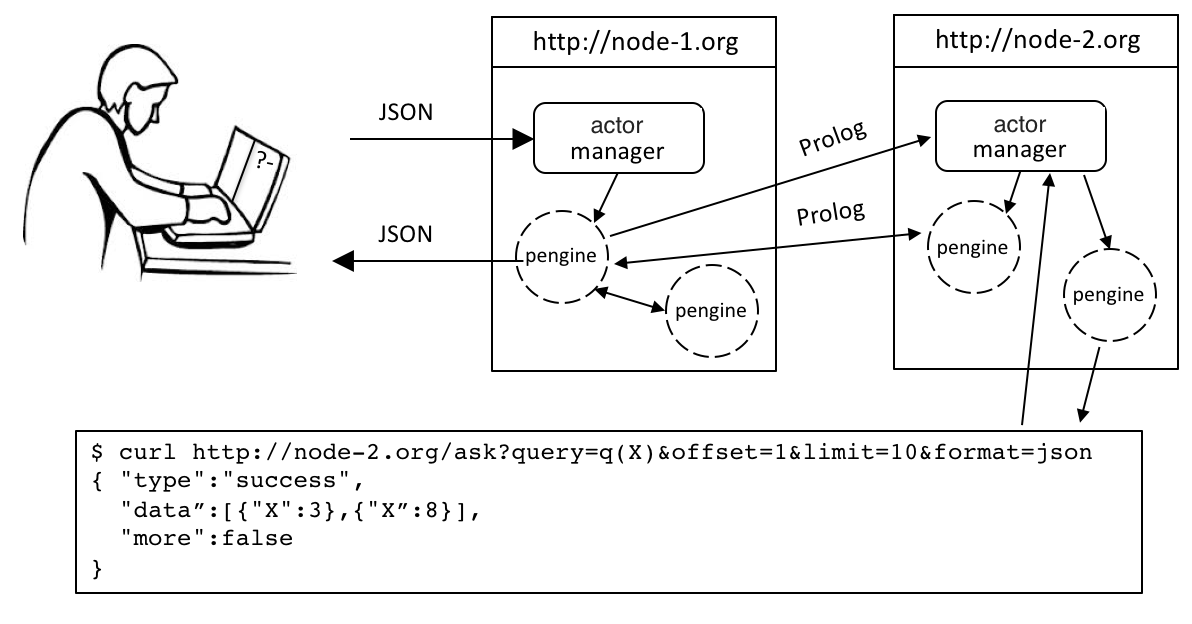
\includegraphics[width=8cm]{swish-pengine-interaction-2}
%    \caption{Mediated by the shell, a programmer controls a small \textit{multi-actor system} consisting of just three pengines. Another client is accessing a fourth pengine by means of an HTTP request to the node at \texttt{http://node-2.org}.}
%    \label{fig:swish-pengine-interaction-2}
%\end{figure}
%
%A node has a dual identity: as a Web Prolog runtime system, and as a node in the network forming the Prolog Web.
%
%--- 
%
%Extension of the Web.
%
%
%
%\subsection{Pure Web Prolog and the pure Prolog Web}
%
%A Prolog program consisting of only Horn clauses is said to be \textit{pure}. It seems reasonable to describe \texttt{rpc/2-3} as a predicate that is pure, at least as long as the goal getting called in the second argument is pure. 
%
%Interestingly, rpc/2-3 retains the logical purity of the predicates it calls.\footnote{This is true also of the \texttt{call/N} family of Prolog predicates.} Indeed, the following seems to hold:
%
%\begin{center}
%\textit{Pure Web Prolog = Pure Prolog + \texttt{rpc/2-3}}
%\end{center}
%
%\noindent With a large number of nodes running pure Web Prolog programs interlinked to other pure Web Prolog programs, we may \textit{in theory} be able to create a Web of Logic on top of the conventional Web, a layer that can \textit{in principle} grow as big as we want it to grow, and even into a network spanning the whole globe, just like the conventional web has done, while still adhering to the formal (model or proof theoretic) semantics of the pure subset of the Prolog language. In practice, this may never happen, but the \textit{architecture} is there. 
%
%Pure Prolog explores each branch of a search tree independently from other branches, backtracking when failure is encountered. Analogously, on the pure Prolog Web, each \textit{node} is explored independently from other nodes and backtracking is triggered here too when failure is encountered. From the caller's point of view, a call to \texttt{rpc/2-3} in the body of a rule is just another subgoal to process, another search tree to traverse, only this time in a Prolog context different from the context of the caller. 
%
%
%\section{Two levels of abstraction}\label{sec:two-levels}
%
%Looking back at Figure~\ref{fig:prolog_web4} there seems to be a sense in which two \textit{levels of abstraction} have appeared. The contents of the boxes with dashed borders form the \textit{level of logic programs}. Below, we find a \textit{level of communicating pengine processes}. Although these levels are clearly related, to the extent that they can be seen as two sides of the same coin, the level of logic programs is considerably more abstract than the level of the pengine processes. On the lower level, processes are created and destroyed and while they are alive they send messages to each other. Nothing of this kind takes place on the level of logic programs. On this level, entities such as processes, messages and mailboxes do not exist -- they have been abstracted away. (This can be seen most clearly in the definition of \texttt{rpc/2-3} in Section~\ref{sec:non-deterministic-remote-procedure-calls}.)
%
%As we see it, drawing a line between these two levels is just another way to express the distinction between declarative and procedural that so often appears in the story about Prolog. Or, said differently, ``What?'' is specified at the level of logic and the corresponding ``How?'' is handled on the level of abstraction underneath it, i.e. on the level of communicating pengine processes. From a procedural point of view, there is nothing strange about the idea that instructions of the form ``in order to do that, do this, then this ... and finally this'' may involve talking to a pengine on another node. That such conversations can take place ``over the wire'' and in a way that preserves the logic as well as the behaviour of Prolog is perhaps the key insight here. It is just a matter of widening the concept of procedural to also cover communication between processes. 
%
%
%\subsection{The not-so-pure Prolog Web}
%
%By using spawn, send and receive or the \texttt{pengine\_*} predicates there are other ways to distribute a program in Web Prolog, while at the same time making good use of any parallelism that can be found and exploited. But this destroys declarativity and is much harder since it involves dealing with concepts such as pengines, pids and messages explicitly.
%
%According to \cite{vlassis2007concise}, agents that implement different behaviours are often called \textit{heterogeneous}.
%
%
%In our first scenario, the programmer was in control of just one single pengine. In other scenarios, this pengine may in turn be in control of and communicate with other pengines and/or other actors. They may be running sequentially, or concurrently. They may be running on the same node, or be distributed over other nodes. That is, in some scenarios, a programmer is in control of the orchestration of what we will refer to as a \textit{multi-actor system}. (Here we exploit the analogy with so called ``multi-agent systems''.)
%
%
%\subsection{Web Prolog and the \textit{programmable} Prolog Web}
%
%The Prolog Web is a programmable web. In its original form, as a hypertext Web of Documents, the Web was not programmable at all, but this changed fairly early with the introduction of CGI-scripts running on a server that generated documents dynamically, and with JavaScript running on the client. Later, remote procedure calling (XML-RPC, JSON-RPC, SOAP) became prevalent, but the term ``programmable web'' was not used until individuals or organisations started to publish ``open'' (often RESTful) web APIs, inviting programmers to combine them into so called ``mashups'', using JavaScript as glue. While the Prolog Web allows all this, it takes the idea a couple of steps further by allowing the owner of a node to offer clients a complete Web Prolog runtime environment scriptable (another word for `programmable'') by more or less complex queries or by the injection of source code into the pengines or other actors running on the node. The node may or may not be equipped with node-resident programs defining predicates that in addition to the built-in ones may be called by the client. This is another form of programming of the Prolog Web, performed by the owner of a node, rather than by a client.
%
%
%\subsection{An open cluster}
%
%The traditional Web is distributed, decentralised and open. These are traits we want the Prolog Web to also possess. Whereas distribution is nicely conceptualised in the actor model, and nicely handled by an actor programming language such as Erlang, decentralisation and openness require features we choose to rely on the Web as such to contribute. Erlang and most other platforms for distributed programming are not open in the sense that we require. They usually rely on TCP for transport and are, for reasons of security, assumed to be operating in a closed, trusted environment where we directly control the machines we are operating. In other words, when Erlang runs on a \textit{cluster}, it is a cluster that is \textit{closed}. We can think of the Prolog Web as a cluster as well, but one that is \textit{open}. 
%
%
%\subsection{Scalability}
%
%By adopting a computational model capable of scaling out not only to multiple cores on one machine but also to multiple nodes running on multiple machines, by introducing an option allowing clients to limit the number of network roundtrips it takes to run a query to completion, by embracing the WebSocket transport protocol with its low overhead per message, by allowing also for an optional RESTful HTTP web API, and by leaving ample room for old as well as new forms of caching on both clients, nodes and intermediaries, we have made our best to ensure our high hopes for the scalability of the Prolog Web layer are not unfounded.
%
%For a multi-pengine system to be able to scale, nodes must be able to spawn very many pengines, creating and destroying pengines must be fast, and the communication among them efficient. A pengine is a kind of actor, and since actors created by the Erlang virtual machine are famous for having exactly those properties, this is certainly one reason (but not the only one) for us to look closely at Erlang, a language which also happens to be very well positioned to take advantage of the so-called hardware multi-core revolution. 
%
%
%
%\begin{itemize}
%
%\item The humble URI plays an important role on the Prolog Web with URIs pointing to nodes, URIs pointing to actors running on nodes, URIs pointing to answers to queries, and URIs pointing to Web Prolog source code. Such URIs can appear in the arguments of predicates, or as values of options passed in predicates.
%
%\item To be successfully webized, a language and an architecture must exploit the existing web infrastructure. In the case of the Prolog Web, the linking of Web Prolog programs into a network of resources requires an extra-logical infrastructure over and above what is already deemed extra-logical about Prolog. 
%
%\item In an open network such as the Web, security is of utmost importance. Since the existing web infrastructure can provide the Prolog Web with some forms of security, this point is related to the previous point. However, there are other forms of security, more related to the nature of Prolog as such, that must also be supported.
%
%
%\end{itemize}
%
%---
%
%
%\begin{itemize}
%\item A fragmented community -- so let's create 1) an interlingua, and 2) a Prolog Web for the community!
%\item A standard that isn't much liked -- so let's create a new one!
%\item Unpopular -- so let's rebrand it and embark on a marketing effort!
%\item Still a logic programming language -- very similar to Prolog
%\item A better version of SWISH and \texttt{library(pengines)}
%\item Wrapping the Web in logic -- the pure Prolog Web -- the programmable Prolog Web which is compatible with purity), the non-pure Prolog Web, and the concurrent Prolog Web
%\item The means for backtracking over the Web -- we no long need to fake it using long-polling.
%\item The importance of the WebSocket protocol 
%\item The fact that it is more or less traditional Prolog -- it allows us to build on ISO Prolog and also to reuse what's available in the form of textbooks.
%\item The integration of the actor-programming model/message-passing concurrency -- a multi-paradigm PL
%\item The similarity to Erlang -- syntax, (semantics), patterns, books, large community, implementation technology. (Suppose Erlang didn't exist. Actor programming might still be the way to go. But then we would have to invent new syntax. The Erlang connection is important. Prolog has a lot to learn from Erlang.)
%\item The importance of multi-core computing
%\item The tight connection between Web Prolog and the Prolog Web (See Section~\ref{sec:birds-eye-view})
%\item The Prolog Web comes with an architecture (See Section~\ref{sec:architecture})
%\item The promise of an interlingua making real-time interoperability possible 
%\item The promise of a new standard for Prolog - easily done through a W3C community group
%\item Simplicity
%\item The relation to the Semantic Web
%\item The importance of online IDEs.
%\item Great for building conversational systems
%\end{itemize}
%
%\begin{description}
%
%\item[Web Prolog is a logic programming language] Based on formal logic, a subject dating all the way back to the antiquity and tried and tested by generations of logicians and philosophers, logic programming forms a paradigm of it own. Even in its pure form, as a set of Horn clauses, Web Prolog is Turing complete. Adding negation as failure gives us an expressive form of non-monotonic logic. Thus, Web Prolog represents a programming paradigm which at its core is unique and very different from JavaScript and other imperative, object-oriented or functional languages that aspire to become web programming languages. 
%
%\item[Web Prolog is a dialect of Prolog] Prolog can be characterised as a logic programming language with imperative and procedural features added to ensure its usefulness as a general-purpose programming language. Prolog is still the best known and most frequently used logic programming language and almost fifty years of logic programming research has not been able to replace it. We know of no other logic programming language mature enough to aspire to the role we want to give Prolog on the Web. It is furthermore the only logic programming language that has been standardised, giving us something to build on in our attempt to adapt Prolog to the Web and create a W3C standard for it. 
%
%\item[Web Prolog is an extension of Prolog] The turn of software toward concurrency, distribution and interaction calls for conceptually extending and evolving programming languages with proper high-level features to tackle these aspects. The choice of an Erlang-ish approach to the actor programming model seems to give us all we need.
%
%\item[Web Prolog is a dialect of Erlang] We admit seeing Web Prolog as a dialect of Erlang may be stretching the notion of a ``dialect'' a bit too far, but we think it is possible to think of it as a variant of the Erlang language where we have ``plugged out'' its sequential part and ``plugged in'' sequential Prolog instead. Consider the syntactic, semantic and pragmatic similarities between Web Prolog and Erlang: dynamic typing, assign-once variables, reliance on pattern matching and recursion, and also the fact that the difference between a function and a relation is not all that big, since the former is a special case of the latter. Consider also the Web Prolog primitives for spawning and messaging that are borrowed straight from Erlang. Admittedly, Erlang has a different focus than Web Prolog -- a focus on fault tolerance and very efficient concurrent programming -- but the fact still remains: while it would be silly to claim that (say) JavaScript is a dialect of Erlang, claiming this for Web Prolog is much more reasonable.
%
%\item[Web Prolog is an extension of Erlang] Seen as an Erlang dialect, Web Prolog has many features not found in standard Erlang, features it inherits from traditional Prolog: built-in backtracking search, unification, logic-based knowledge representation and reasoning, meta-programming, user defined operators, a term expansion mechanism and definite clause grammars. Furthermore, Web Prolog tries to be more open than Erlang -- open in the sense the Web is open. Indeed, if it was not for the fact that Web Prolog resembles Prolog a lot more than it resembles Erlang, we might have named it ``Web Erlang''.
%  
%\item[Web Prolog is an embedded language] Just like JavaScript, and in contrast to traditional Prolog and Erlang, Web Prolog is an embedded language, a language designed to be implemented in a host language running in a host environment. We have embedded our Web Prolog proof-of-concept implementation in SWI-Prolog, making good use of the libraries this platform provides, but we are convinced it can also be embedded in other Prolog systems, in systems supporting non-Prolog programming languages or knowledge representation languages, and possibly also in web browsers through transpilation into JavaScript or compilation of the Prolog runtime into WebAssembly.
%
%\item[Web Prolog is a sandboxed language] Just like JavaScript, in support of openness and in contrast to traditional Prolog and Erlang, Web Prolog is a sandboxed language, open to the execution of untested or untrusted source code, possibly from unverified or untrusted clients without risking harm to the host machine or operating system. Therefore, Web Prolog does not include any predicates for file I/O, socket programming or persistent storage, relying for these upon the host environment in which it is embedded. Access to the node's host environment can only be granted by the owner who can implement new predicates in the host language and import them into the program space of the node. The author of such code must take responsibility for any security issues that may arise as a consequence of such imports.
%
%\item[Web Prolog is a scripting language] Just like JavaScript, and in contrast to traditional Prolog and Erlang, Web Prolog sometimes plays the role of a scripting language. The best example of scripting probably is when a client injects a (usually small) chunk of Web Prolog source code into a pengine or other actor created on a remote node, thus adding to the context in which subsequent queries by this client are to be evaluated. Note that in contrast with JavaScript, the client is scripting the server, rather than the other way around. Of course, this is exactly what is involved in ``bringing code to the data''. Doing it the other way around, i.e. ``bringing data to the code'' is also possible. Indeed, there is an useful symmetry here, allowing Web Prolog code to flow in either direction, from the client to the node or from the node to the client. The choice is determined by the programmer's selection of combinations of options that will configure the actor to be created, but the choice can in principle also be made programmatically at runtime.
%
%\item[Web Prolog is an interactive-mode language] Similar to other scripting languages, Web Prolog is an \textit{interactive-mode language}, allowing programmers to enter queries one at a time in a shell, and to see the result of their evaluation immediately. This is already a well-known and much appreciated feature of traditional Prolog. In a Web Prolog shell the interactive-programming mode has been extended with \texttt{flush/0} for inspecting the content of the mailbox of the top-level pengine to which the shell is attached, a feature it borrows from Erlang.
%
%
%\item[Web Prolog is a knowledge representation language] Similar to most other scripting languages, Web Prolog can be used for purposes for which ``scripting'' is not really the right word. Using Web Prolog, the owner of a node is for example able to build knowledge bases consisting of millions of clauses -- facts as well as rules. (This, obviously, depends a lot on the actual capability of the node in question. For our SWI-Prolog implementation it would be true.) However, as a knowledge representation system, although it subsumes relational as well as deductive databases, Prolog (and Web Prolog) as such it is rather weak in terms of expressiveness. But there is also negation as failure -- an important extension allowing non-monotonic knowledge representation -- and with its core based on logic, Web Prolog is rather well suited for interfacing to other logic-based languages of the knowledge representation world such as languages for constraint logic programming, abductive logic programming, probabilistic logic programming and disjunctive logic programming.
%
%
%
%\item[Web Prolog is an ultra-high-level programming language] This is an epithet we think it deserves due also to the way options are used to ``configure'' pengines (or other actors) to be run, some of which are there to inject source code into the actor, while others are pragmas which are there to influence the way the processing and communication are performed.
%
%
%\item[Web Prolog is an actor programming language] With the addition of predicates for Erlang-style message-passing concurrency  it is reasonable to claim that Web Prolog is an \textit{actor programming language}. In any case, we think that if we are prepared to say that Erlang is an actor programming language (and some may hesitate to do that), then we must be prepared to say that so is Web Prolog. All the machinery that matters for programming systems of actors are there, behaving in a way which is consistent with how it works in Erlang, yet implements a very comprehensive Prolog dialect as well. 
%
%\item[Web Prolog is a distributed programming language] The advent of massive concurrency through multi-core computer architectures has revived interest in the actor model. Through Erlang (and Elixir) this model has been shown to work extremely well in practice. The actor model, providing us with a single abstraction as a solution to the two problems of concurrent and distributed programming, is a key ingredient in our proposal. The ``high-level distributed programming facilities'' was mentioned in the quote in Section~\ref{sec:p-kind}, and they may have existed at the time (Linda? April?), but, as we see it, it is not until now that we, thanks to the WebSocket protocol, can hope to implement something adapted to the Web as well as to the future of networked multi-core hardware.
%
%\item[Web Prolog is an agent programming language] The notion of an agent is rather fuzzy but there are at least three properties most theorists would agree a software agent must possess: it must be a process of a sort, only loosely connected to other processes, it must be stateful, thus have a kind of memory of its own, and it must be capable of interacting with the world external to it. Note that under this definition, any stateful actor would qualify as an agent, and even Erlang might be seen as an agent programming language. A pengine is a kind of actor which in addition to the properties listed above has two other traits we intuitively tend to associate with agenthood: it is capable of reasoning and capable of giving answers to queries -- answers that follow logically from what it believes. So if Erlang is an agent programming language, then this must certainly be true of Web Prolog as well. 
%
%\item[Web Prolog is an agent communication language] All communications between a client and a node is couched in the language of Web Prolog, allowing us to think of it as an \textit{agent communication language} (ACL). Compared to standardised ACLs such as FIPA-ACL and KQML, which both define a set of \textit{communicative acts} inspired by speech act theory, Web Prolog is of course much cruder. But the act of asking for the first answer to a query (using \texttt{pengine\_ask/2-3}) and the act of asking for the next answer to the same query (using \texttt{pengine\_next/1-2}) would certainly remind a linguist interested in pragmatics of communicative acts. Even clearer examples can be found in the distinction between statements and questions, and, among the questions, the distinction between Yes/No questions just checking if a ground query is true or false, and WH questions asking for variables in non-ground queries to be bound. In the field of expert systems, Why and How questions asking for explanations have also played a role. Other kinds of actors, using protocols other than the PCP, may make use of other systems of communicative acts.
%
%\item[Web Prolog is a multi-agent programming language] If we choose to look upon a pengine as a simple kind of agent, then it is of course also reasonable to view Web Prolog as a language for programming a \textit{simple} kind of multi-agent systems (MASs). However, we prefer to use the term \textit{multi-pengine systems}\footnote{The other alternative term \textit{multi-actor systems} seems to be taken already. See e.g.:\\ \url{https://www.tudelft.nl/en/tpm/about-the-faculty/departments/multi-actor-systems/} } instead, and although it resembles a multi-agent language, we are therefore tempted to describe Web Prolog as \textit{multi-pengine programming language} instead.
%
%
%\item[Web Prolog is an NLP programming language] Prolog was created as a language intended for natural language processing (NLP) and still is the only (major) programming language with a built-in unification-based grammar formalism. A particular kind of agents for which Web Prolog due to its roots in natural language processing might be a suitable implementation language for is the so called conversational agents.
%
%\noindent [FIXME: Write something about Colmerauer, Pereira and Shieber? Relate to NLTK?]
%
%\item[Web Prolog is a robotics programming language] ...
%
%\end{description}
%
%---
%
%Other clients may use HTTP instead of websockets, but this, as we shall see, comes at the price of only being able to use a more constrained version of the PCP protocol. 
%
%---
%
%\subsection{The stateless HTTP API}
%
%An IDE for traditional Prolog is a fairly demanding type of web application. Although the conversation between the programmer and the pengine must always be initiated by the programmer using the shell, the interaction may at any point turn into a mixed-initiative conversation driven by requests for input made by a running query. What makes unconstrained mixed-initiative interaction feasible is the support for efficient bi-directional messaging offered by a node thanks to the use of the WebSocket protocol.
%
%Other kinds of web applications put less demands on a node and may be happy treating it as a mere ``logic server'', and thus have no need for mixed-initiative interaction. Then HTTP may suffice.
%
%In contrast to WebSocket, HTTP is a stateless protocol, meaning that each request message must be understood in isolation. This means every request needs to bring with it as much detail as the server needs to serve that request, without the server having to store a lot of information from previous requests. 
%
%The HTTP API that offers access to an arbitrary Web Prolog node is based on the realisation that URIs of the following form constitute a generic Prolog solver API which is in several ways ideal:
%
%\begin{lstlisting}
%<BaseURI>/ask?query=<Query>&offset=<N>&limit=<L>
%\end{lstlisting}
%
%\noindent Such URIs are simple, they are meaningful, they are declarative, they can be bookmarked, responses are cachable by intermediates, and so on. We would therefore suggest that \textit{any} attempt to come up with a generic HTTP API to Prolog should take the form of such URIs as its point of departure.
%
%Here is how we ask for the first solution to a query:
%
%\begin{lstlisting}
%GET http://remote.org/ask?query=mortal(X)&offset=0 
%\end{lstlisting}
%
%\noindent As over the WebSocket connection, solutions are given as Prolog or as Prolog variable bindings encoded as JSON. To ask for the next two solutions, we can make a new GET request, setting \texttt{offset} to \texttt{1} this time and adding a parameter \texttt{limit=2} to the request.
%
%A naive implementation of this web API would be inefficient since the second request would have to recompute the solution returned by the first request. 
%
%
%
%---
%
%The actor model provides us with one single abstraction as a solution to the two problems of concurrency and distribution; it allows applications to scale out not only to multiple cores on one machine but also to multiple nodes running on multiple machines on a network such as the Internet.
%
%In Web Prolog each actor is equipped with its own workspace, a dynamic database private to it. As long as the actor process is alive, a client is allowed to update the workspace using predicates such as \texttt{assert/1}, \texttt{retract/}1 and \texttt{retractall/1}. Updates must be performed via messaging -- a client basically must ask the actor to update itself -- and they will only affect that actor's workspace, not actors running elsewhere, and not even actors running on the same node. This means that problems caused by two or more processes trying to update the same database simultaneously cannot arise. Keep in mind that since database updates performed by one process is not seen by other processes, assert and retract cannot be used for inter-process communication. Web Prolog adheres to the idea that processes should ``communicate to share memory, rather than share memory to communicate''.
%
%Therefore, although the following goal is permitted, it is quite meaningless since the clause \texttt{foo(a)} disappears as the goal has run and the spawned process has terminated.
%
%\begin{lstlisting}
%?- spawn(assert(foo(a)), Pid).
%Pid = '75a7715c-64b8-11e7-aed5-8bb40804b542'.
%?-
%\end{lstlisting}
%
%\noindent The dynamic database gives us an alternative way to maintain the state of an actor.
%
%Actors can be scripted. That is how we as programmers tell them what to do while they are alive -- what messages to listen for, and what messages to send in order to make things happen. As we shall see, an actor may for example be programmed to simulate a refrigerator capable of understanding messages such as ``store food'' and ``take food''. More importantly, and as we will show as well, an actor can be programmed to provide answers to questions -- answers that follow logically from what the actor knows.
%
%
%The logic programming model...
%
%An actor can be seen as the fundamental computational unit in a \textit{combined} logic-based and actor-based model of computation. Since it implements SLD resolution we can think of it as a reasoning engine, and by virtue of its ability to send and receive messages we can think of it as an interaction engine. An actor adheres to the laws of logic and to the norms of its communication protocol -- it is both a reasoning engine and an interaction engine.
%
%A pengine is a special \textit{kind} of actor characterised by a particular communication protocol -- the Pengine Communication Protocol (PCP). We shall return to the details of the PCP further below, but for now it suffices to say that this protocol is basically what makes a pengine into a first-class Prolog top-level. We can send it queries, and be sent answers in return, answers that follow logically from the ``beliefs'' that the pengine holds. In this sense, a pengine is an interactive reasoning engine. Similar to a normal Prolog top-level, a pengine is ``lazy'' in the sense that it will not produce all the answers to a query at once, unless we explicitly ask it to do so. Typically, we send it a query and get one answer back. Then we send it a request for another answer to the same query, and if there is one, we get it too. At any point in the conversation, we may choose to stop asking for more answers to the first query, and to send it a different query instead, and so on. We can think of this as an \textit{ask-next-stop} kind of protocol.
%
%As we shall see, a node supports another and very different protocol as well, based on integer offsets into a virtual index of solutions to queries rather than relying on the \textit{ask-next-stop} idea. Using this protocol, and given a query, we are always able to ask for the solution at offset \textit{i}, regardless of the value of \textit{i}. It also means we can choose to query a node \textit{directly}, rather than to query a particular pengine running on the node. As it is a stateless protocol, and thus nicely captures the notion of so called \textit{RESTfulness}, this has certain implications for the scalability of the Prolog Web.
%
%---
%
%Sofware development methodology: Erlang's contribution here concerns not only reactiveness but also the orchestration of concurrent and possibly distributed processes using message passing. As suggested by \cite{Armstrong2003}, it allows us to organise our system as a set of communicating processes. By enumerating all the processes in our system, and defining the message passing channels between them, we can partition the system into a number of well-defined components which can be independently implemented and tested.
%
%---
%
%The notions of actors and pengines are  key to the architecture of what we think of as \textit{the Prolog Web}. 
%
%The Prolog Web, as we envision it, will share traits such as distribution, decentralisation and openness with the traditional Web. It will also share some traits with the Semantic Web, but at its core be based on Horn clause logic, a logic that is simpler and less expressive than the description logic on which the Semantic Web is based.
%
%One might think of the Prolog Web as the Web raised to a new level of abstraction, a level on which logic has become an integral part, but where programming still counts for something. Another way to put it is to say that we are \textit{wrapping the Web in Prolog}, which, since Prolog is a logic programming language, implies that we are wrapping it in \textit{logic}.
%
%A \textit{node} is an executing Web Prolog runtime environment that has been given a unique name in the form of a URI. Its purpose is to host pengines and other kinds of actors. A node is equipped with a comprehensive set of web APIs, using both WebSocket and HTTP as transport protocols, over which a client can run Web Prolog programs defined by the owner of the client, the owner of the node, or by contributions from both. A node has a dual identity: as a Web Prolog runtime system, and as a node in the network forming the Prolog Web.
%
%---
%
%Erlang and Prolog are both general-purpose programming languages.
%
%\begin{figure}[h]
%    \centering
%	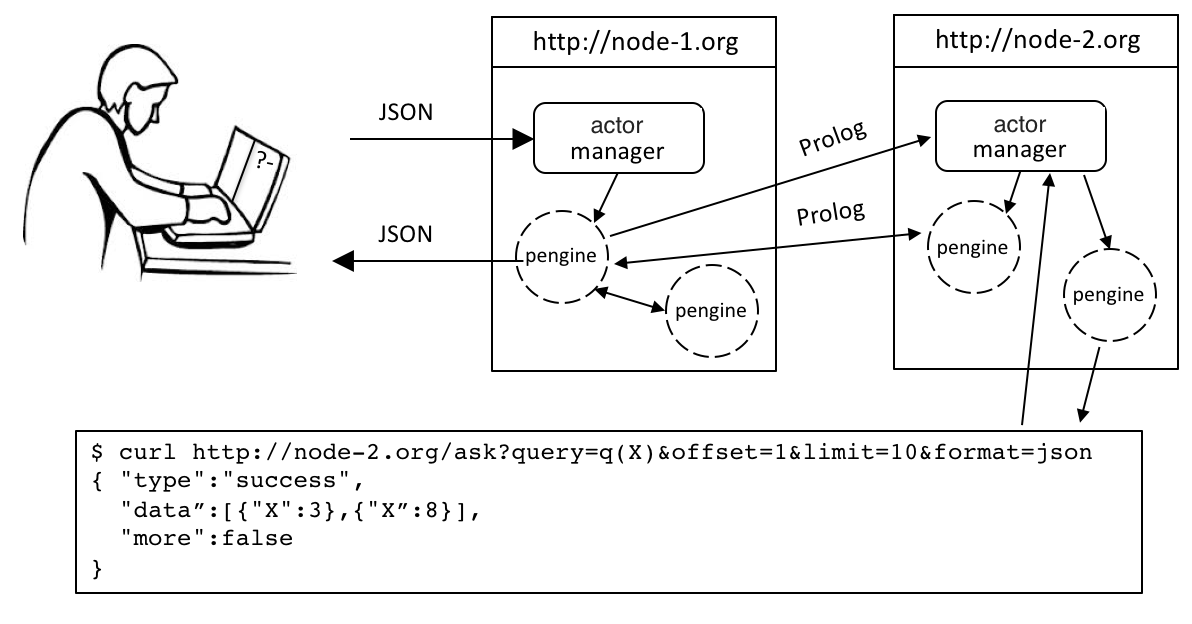
\includegraphics[width=8.5cm]{swish-pengine-interaction-2}
%    \caption{Mediated by the shell, a programmer controls a small \textit{multi-actor system} consisting of just three pengines. Another client is accessing a fourth pengine by means of an HTTP request to the node at \texttt{http://node-2.org}.}
%    \label{fig:swish-pengine-interaction-2}
%\end{figure}
%
%\noindent The task of the \textit{actor manager} is to handle the reception of messages sent by clients and arriving over HTTP and WebSocket connections. They may be messages requesting the spawning of a pengine or termination of a pengine, or messages to be forwarded to the pengine addressed by a pid. The actor manager is also responsible for the registration and deregistration of pengines. The registration happens right after the creation of a pengine, deregistration after it has terminated.
%
%Despite what Figure~\ref{fig:swish-pengine-interaction-2} may suggest, the programmer may not be alone in interacting with this particular node. Other programmers may be talking to other actors running on the same node. The actors are completely shielded from each other, unless of course the programs they are running have been written to allow them to communicate. In any case, actors do not share memory, so in order to share information, they must exchange messages.
%
%Crucially, a node may also host a Web Prolog \textit{program} -- a database, an expert system, a game engine, a digital assistent, a home control system, or another kind of program. If it does, any pengine running on the node has access to the predicates defined by this program. The program -- which we shall refer to as the \textit{node-resident} program -- is typically maintained by the owner of the node. Unless we are authorised to do so, we are not able to make any changes to it, only the owner is allowed to do so. However, by means of code injection in the workspace of the pengine, we are allowed to \textit{complement} the node-resident program with source code we have written ourselves. Another way to put it is to say that we are \textit{programming} the pengine, which in turn leads us to our claim that the Prolog Web is \textit{programmable} in a sense stronger than the usual.
%
%---
%
%We thus have three levels of abstractions: the \textit{actor}, the \textit{pengine} (built on top of an actor) and the \textit{non-deterministic remote procedure call} (built on top of a pengine). In addition, we may want to treat the \textit{node} as a fourth abstraction (also built on top of the pengine abstraction). In chapters that follow we intend to show how these abstractions are related.
%
%---
%
%The syntax of Erlang is very close to the syntax of Prolog, and it made sense to take advantage of this when designing Web Prolog. After all, making Erlang programmers feel at home with Web Prolog could turn out to become just as important as making Prolog programmers feel at home with the language.
%
%This chapter presents a number of programming examples. The majority of the examples are there to show that Web Prolog programs can be written in the style of Erlang, whereas the ones towards the end of the chapter show how to deal with the non-determinism not present at all in Erlang.
%
%A number of Web Prolog programming patterns inspired by similar patterns in Erlang will also be demonstrated: The use of concurrency and recursion for maintaining state, the use of protocols, and various abstractions for asynchronous and synchronous communication between processes, just to mention a few examples. Patterns based on failure-driven loops -- a concept foreign to Erlang but well-known in Prolog -- will be demonstrated as well. On a higher level, the implementation of two communication models, \textit{request-response} and \textit{publish-subscribe}, will also be demonstrated.
%
%\section{Traditional Prolog}
%
%Suppose we (inspired by events said to have taken place around the times when logic was born) have written the following program in the editor:
%
%\begin{lstlisting}
%mortal(X) :- human(X).
%human(X) :- featherless(X), biped(X).
%featherless(socrates). 
%featherless(plato). 
%featherless(diogenes).
%biped(socrates). 
%biped(plato). 
%biped(diogenes).
%\end{lstlisting}
%
%\noindent Turning then to the shell, we consult the content of the editor, enter a query and inspect the results produced by the Prolog top-level, one-at-a-time in the usual lazy fashion:
%
%\begin{lstlisting}
%?- mortal(X).
%X = socrates ;
%X = plato ;
%X = diogenes.
%?-
%\end{lstlisting}
%
%Pure Prolog (Horn clauses). SLD resolution -- the depth-first traversal of the search tree and the use of backtracking when failure nodes are encountered. 
%
%Web Prolog is a logic programming language. Based on formal logic, a subject dating all the way back to the antiquity and tried and tested by generations of logicians and philosophers, logic programming forms a paradigm of it own. Even in its pure form, as a set of Horn clauses, Web Prolog is Turing complete. Adding negation as failure gives us an expressive form of non-monotonic logic. Thus, Web Prolog represents a programming paradigm which at its core is unique and very different from JavaScript and other imperative, object-oriented or functional languages that aspire to become web programming languages. 
%
%AI-related tasks such as knowledge representation and problem solving, and applications such as expert systems and natural language processing.
%
%General-purpose programming language.
%
%
%\section{Web Prolog}
%
%Starting from traditional Prolog, we take what might be called a \textit{shrink-and-extend approach} to the design of Web Prolog. We shrink Prolog by removing primitives that do not seem to ``belong'' on the Web, and we extend it with carefully crafted primitives heavily inspired by Erlang, as well as with APIs useful for building web applications. We are aiming for a fairly small language, so we try to extend by less than we shrink.
%
%
%\section{Inspirations from Erlang}
%
%Erlang was designed with the aim of improving the development of telephony applications, but has in recent years, thanks to its built-in support for massive concurrency, distribution and fault tolerance, been used as a very capable language for implementing the server-sides of web applications.
%
%Erlang processes are implemented by the virtual machine, not by operating system threads. They are very lightweight, and completely isolated from each other. Creating and destroying processes is very fast, and millions of processes can be created on one machine. Sending messages between processes is also very fast. Therefore, in the context of the Web, Erlang provides the advantage that we can have one server process per web client, or (say) ten of them if we want.  We hasten to add that while we do not aim for the kind of \textit{massive} concurrency Erlang is known for, we certainly do our best not to introduce features in the Web Prolog language that would make massive concurrency impossible.
%
%The design of Web Prolog takes a lot of inspiration from Erlang, and primitives for process creation and messaging makes Erlang-style concurrent programming possible. As we shall see, an Erlang-style actor-based architecture for Web Prolog and the Prolog Web also creates something of a semantic foundation for the Prolog Web. On top of actors, we shall build pengines, and using pengines we shall implement web APIs as well as a simple yet powerful predicate for making non-deterministic remote procedure calls. 
%
%Erlang and Prolog are in many ways similar. Most data types map cleanly between the two languages. Atoms are the same in Erlang and Prolog, and the same goes for integers and floating point numbers. Lists look and behave the same in Prolog and Erlang, and an Erlang tuple \texttt{\{foo,a,1\}} corresponds most naturally to a Prolog term \texttt{foo(a,1)}.\footnote{However, note that \texttt{\{foo,a,1\}} is a term in Prolog too, of the form \texttt{\{\}((foo,(a,1)))}} Furthermore, Prolog variables are assign-once variables, just like Erlang variables, pattern matching is the dominant way to pass values, just like in Erlang, and just like in Erlang, loops are normally implemented by means of recursion.  
%
%The most important difference between the two languages is of course the fact that Erlang is a functional language, whereas Prolog is relational. Since a function is just a special case of a relation this difference must not be exaggerated, but it does show in the way function calls may be nested, something that cannot be done in Prolog since arguments are used to represent outputs as well as inputs.\footnote{One can of course build a preprocessor than translates functional notation into the relational syntax of Web Prolog.}
%
%The following listings of Prolog code (to the left) and Erlang code (to the right) show some of the similarities as well as some of the differences between the two languages:
%
%\begin{lstlisting}
%% length                       % length              
%
%length([], 0).                 length([]) -> 0;      
%length([_|T], N) :-            length([_|T]) ->      
%    length(T, N1),                 1 + length(T).    
%    N is N1 + 1.                                             
%\end{lstlisting} 
%
%\noindent The Erlang program is even Prolog readable.
%
%It is sometimes lamented that the inventors of Erlang should have chosen a more ``traditional'' syntax -- it is quite unlike what most programmers are used to and is a hurdle to cross. Prolog programmers do of course beg to differ -- we are fine with the syntax. What we do not like has more to do with semantics and the sacrifice of a lot of good things that Prolog has to offer. It can hardly be denied that some very useful features were lost somewhere on the road from Prolog to Erlang.\footnote{There is even a talk by Joe Armstrong on YouTube, where he seems to be regretting removing too much Prolog from Erlang. See https://www.youtube.com/watch?v=h8nmzPh5Npg\#t=40m17s} Here is an attempt to list those features that are available in Prolog (and in Web Prolog) but not in Erlang:
%    
%\begin{itemize}
%\item
%  Built-in backtracking  search
%\item
%  Unification
%\item
%  Logic-based knowledge representation
%\item
%  Reasoning
%\item
%  Meta-programming
%\item
%  User defined operators
%\item
%  A term expansion mechanism
%\item
%  Definite Clause Grammar (DCG)
%\end{itemize}
%
%
%\noindent Those are some powerful features that were removed from Prolog in order to arrive at Erlang. In no way should this be seen to imply that we think that the inventors of Erlang made a \emph{mistake} when they scrapped Prolog in favour of a simple functional language. Given that Prolog is fairly difficult to learn and to use correctly, given the nature of the problems with programming telephone switches that they set out to solve, and perhaps in an attempt to avoid being dragged down by the post fifth generation dismissal of logic programming, they probably made the right decision. After all, Erlang is a very successful programming language, far more successful than Prolog, and this is the proof of the pudding. 
%
%For Web Prolog, the similarity with Erlang goes deeper than syntax or data types. Just like Erlang but in contrast to ISO Prolog, Web Prolog is an \textit{actor-based language}. 
%
%\section{Running Web Prolog from/in a browser}
%
%What does it mean to be a web programming language? One way to characterise a web programming language is to say that it can be \textit{used from} a web browser. Another way to characterise a web programming language is to say that it can be \textit{run in} a web browser.
%
%We anticipate that, in a not-too-distant future, robust and efficient implementations of Prolog will appear which will run in clients such as web browsers, and thus provide an alternative to JavaScript there. With languages such as Elm and ClojureScript, functional programming is moving in this direction. At least one leading engineer at Google thinks we need more web programming languages.\footnote{\url{https://www.pcworld.com/article/2362500/google-engineer-we-need-more-web-programming-languages.html}} When it comes to web logic programming languages, not much is going on. We hope and believe that Web Prolog could eventually become such a language.
%
%\begin{figure}[h]
%    \centering
%	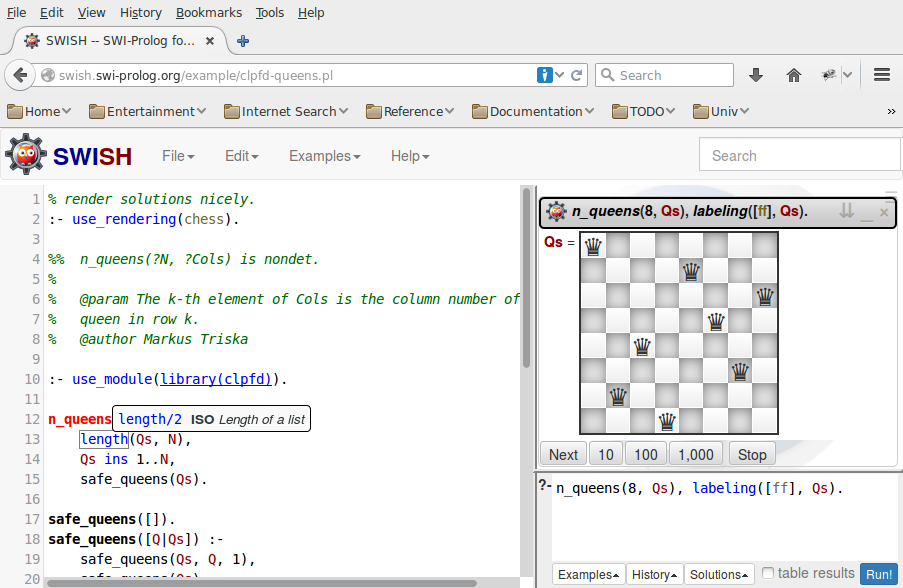
\includegraphics[width=8cm]{swish}
%    \caption{The Web Prolog proof-of-concept implementation.}
%    \label{fig:swish-first}
%\end{figure}
%
%\noindent We have implemented the core Web Prolog predicates as well as a minimal node in SWI-Prolog \cite{wielemaker:2011:tplp}, effectively using SWI-Prolog as an informal but executable specification language. 
%
%
%SWISH 
%
%Running the program examples in a shell in a browser. 
%
%
%\section{Two kinds of web APIs}
%
%Web APIs play a central role on the Prolog Web. Not only do they allow a non-Prolog client -- typically implemented in JavaScript and built to be run in a web browser -- to create and communicate with a pengine running on a remote node, but they also allow this pengine to talk to \textit{other} pengines on the Prolog Web, thus forming a multi-pengine system capable of utilising local as well as remote resources for satisfying the information and/or control needs of the user running the client. The only reliable way to interact with a node is to use the web APIs it provides.
%
%We focus on two transport protocols in particular: WebSocket and HTTP. We did not have much choice here, since if we do not use HTTP or WebSocket, we simply are not on the Web. Having been developed to serve communication on the Web, these protocols are characterised by their ability to traverse firewalls and to play nicely with proxies. Using these protocols, rather than developing our own is, alongside the addressability of resources provided by URIs, another way to ensure the openness of the Prolog Web.
%
%For maximal flexibility nodes on the Prolog Web offer two kinds of APIs: 1) an asynchronous and stateful WebSocket API, and 2) a synchronous and stateless HTTP API. In this section we will take a closer look at them, describe how they differ, and demonstrate how they can be used.
%
%\subsection{The WebSocket API}
%
%In order to enable a client to control all aspects of a set of pengines and other actors, a node offers a WebSocket sub-protocol. WebSocket is a real-time, low latency, bi-directional protocol for asynchronous communication between a client and a server. The WebSocket protocol differs from TCP in that it enables a stream of messages instead of a stream of bytes. With websockets, data is always sent as a whole message. The receipt of a message is event driven and the data payload in an event is always the entire message the other side sent. Under the hood, websockets is built on top of normal TCP sockets.
%
%For Web Prolog, all of this works to our advantage since we specifically want to use the message passing type of paradigm that the WebSocket protocol offers. Thus, being already message-based, websockets save us from most of the work involved in implementing (for example) the PCP protocol.
%
%By their nature of being initiated via an HTTP connection which is then switched over to the WebSocket protocol, websockets can operate on the same port as an HTTP server. There is a vast infrastructure for HTTP and HTTPS that already exists (proxies, firewalls, caches, and other intermediaries), ensuring that security requirements of the modern web are fulfilled and the browser and the node can validate each other.
%
%In addition, we want web browsers to be able to connect to our nodes, and browsers do not support plain TCP, only HTTP requests and WebSocket connections. Also, other types of clients can easily use a WebSocket connection, arguably more easily than they would be able to use a custom protocol built on top of TCP.
%
%WebSocket client libraries are available for the most common general programming languages. In all the major web browsers, the WebSocket object provides a JavaScript API for creating and managing a WebSocket connection to a server, as well as for sending and receiving data on the connection.\footnote{See \url{https://www.w3.org/TR/websockets}} The role of JavaScript here is to construct a new websocket, to define the necessary handlers for \texttt{onopen}, \texttt{onmessage}, \texttt{onerror} and \texttt{onclose} messages, and to call methods for sending messages or closing the connection. A synopsis that leaves out a lot of details can be given as follows:
%
%\begin{description}
%\item[Constructor]
%\begin{lstlisting}
%
%var ws = new WebSocket(<URI>[,<protocol>);
%\end{lstlisting}  
%
%\item[Event listeners]
%\begin{lstlisting}
%
%ws.onerror = function(message) {...}
%ws.onopen = function(message) {...}
%ws.onmessage = function(message) {...}
%ws.onclose = function(message) {...}
%\end{lstlisting} 
%
%\item[Methods]
%\begin{lstlisting}
%
%ws.send(message)
%ws.close()
%\end{lstlisting}  
%
%\end{description}
%
%
%\noindent The messages that are used to spawn pengines or other actors as well as messages that can be used to control them are stringified JSON. Given a connection, and somewhat schematically, spawning a pengine is done like so, where the options part is optional:
%
%\begin{lstlisting}  
%connection.send(JSON.stringify({
%  command: 'pengine_spawn',
%  options: <options>
%}));
%\end{lstlisting}  
%
%\noindent By design, the messages understood by the PCP sub-protocol matches the \texttt{pengine\_*} predicates quite well. Subject to options, answers and other kinds of messages arriving from the node are returned in the form of JSON or Prolog text. Client code written in JavaScript would normally request that they be encoded in JSON. The pid of the created pengine is returned to the client, not in the form of the binding of a variable (as in the predicate API), but in the form of a message \texttt{\{"type":"spawned","pid":<pid>\}}. 
%
%Given the pid, we can ask a query by sending a message which exactly reflects the \texttt{pengine\_ask/2-3} predicate in the predicate API:
%
%\begin{lstlisting}  
%connection.send(JSON.stringify({
%  command: 'pengine_ask',
%  pid: <pid>
%  query: <query>,
%  options: <options>
%}));
%\end{lstlisting}  
%
%\noindent The full set of options valid in the predicate API is valid in the web API as well. In the message corresponding to \texttt{pengine\_spawn/2} we can use options such as \texttt{exit}, \texttt{monitor}, \texttt{link}, \texttt{timeout}, \texttt{src\_predicates}, \texttt{src\_list}, \texttt{src\_text} and \texttt{src\_uri}. (Recall that the majority of these options are inherited from \texttt{spawn/3}.) For \texttt{pengine\_ask/3} we can use \texttt{template}, \texttt{offset} and \texttt{limit}. For \texttt{pengine\_next/2} there is only one valid option, namely \texttt{limit}.
%
%
%\subsection{A comprehensive WebSocket example}
%
%As an example of how the WebSocket API can be used from JavaScript the following code will create a WebSocket connection to a node, spawn a pengine there, and (when having received a pid) ask the query \texttt{mortal(Who)} and retrieve the answers one by one:
%
%\begin{lstlisting}
%var ws = new WebSocket('ws://remote.org/ws','PCP');
%ws.onopen = function (message) {
%  ws.send(JSON.stringify({
%    command: 'pengine_spawn',
%    options: '[format(json)]'
%  }));
%};
%ws.onmessage = function (message) {
%  var event = JSON.parse(message.data);
%  if (event.type == 'spawned') {
%    ws.send(JSON.stringify({
%      command: 'pengine_ask',
%      pid: event.pid,
%      query: 'mortal(X)'
%    }));
%  } else if (event.type == 'success') {
%    console.log(event.data);
%    if (event.more) {
%      ws.send(JSON.stringify({
%        command: 'pengine_next',
%        pid: event.pid
%      }));
%    }
%  }
%};    
%\end{lstlisting}   
%
%
%\subsection{The RESTful HTTP API}
%
%HTTP is the oldest transport protocol for the Web and was, during many years, the only one that counted. It is designed as a simple request-response protocol between a web client and a web server. The client is always initiating the exchange by making a request, whereas the server is responsible for the response. 
%
%In contrast to WebSocket, HTTP is a stateless protocol, meaning that each request message must be understood in isolation. This means every request needs to bring with it as much detail as the server needs to serve that request, without the server having to store a lot of information from previous requests. 
%
%The HTTP API that offers access to an arbitrary node on the Prolog Web is based on the realisation that URIs of the following form constitute a generic Prolog solver API which is in many ways ideal:
%
%\begin{lstlisting}
%<BaseURI>/ask?query=<Query>&offset=<N>&limit=<L>
%\end{lstlisting}
%
%\noindent Such URIs are simple, they are meaningful, they are declarative, they can be bookmarked, responses are cachable by intermediates, and so on. We would therefore suggest that \textit{any} attempt to come up with a generic HTTP API to Prolog should take the form of such URIs as its point of departure.
%
%---
%caching scheme
%---
%
%In a request, only the \texttt{query} parameter is mandatory:
%
%\begin{lstlisting}
%GET <BaseURI>/ask?query=<Query>
%\end{lstlisting}
%
%\noindent Optional parameters accepted are \texttt{template} (default is the variables in the query), \texttt{offset} (default is \texttt{0}), \texttt{limit} (default is \texttt{1}), \texttt{timeout} (default is \texttt{inf}) and \texttt{format} (default is \texttt{json}).
%
%Here is how we ask for the first solution to a query:
%
%\begin{lstlisting}
%GET http://remote.org/ask?query=mortal(X)&offset=0 
%\end{lstlisting}
%
%\noindent As before, solutions are (by default) given in the form of Prolog variable bindings, encoded as JSON. In this case, there is only one binding, of \texttt{X} to the atom \texttt{socrates}:
%
%\begin{lstlisting}
%{ "type":"success", 
%  "pid":"anonymous",
%  "data":[{"X":"socrates"}],
%  "more":true
%}
%\end{lstlisting}
%
%\noindent Note the value \texttt{anonymous} of the \texttt{pid} property. Revealing the pid of the pengine that computed the solutions would perhaps not hurt, but would be potentially misleading since the pengine cannot be used outside the caching scheme.  
%
%The value \texttt{true} of the \texttt{more} property indicates there may be more solutions to the query. To ask for the next solution, we can make a new GET request, setting \texttt{offset} to \texttt{1} this time and adding a parameter \texttt{limit} to the request:
%
%\begin{lstlisting}
%GET http://remote.org/ask?query=mortal(X)&offset=1&limit=2 
%{ "type":"success", 
%  "pid":"anonymous",
%  "data":[{"X":"plato"}{"X":"diogenes"}],
%  "more":false
%}
%\end{lstlisting}
%
%\noindent Sure enough, the node responded with the next solution. The value \texttt{false} shows that there are no other solutions to be found. If we insist anyway, by setting \texttt{offset} to \texttt{3}, we would receive a response of the form \texttt{\{"type":"failure", "pid":"anonymous"\}}.
%
%---
%
%Drawbacks
%
%
%\section{Spawning and messaging in Web Prolog}
%
%Web Prolog offers five core predicates inspired by the corresponding functions in Erlang: \texttt{self/1}, \texttt{spawn/1-3}, \texttt{!/2}, \texttt{receive/1-2} and \texttt{exit/1-2}. Consider the following run of a query involving four of them:
%
%%\begin{lstlisting}
%%?- self(Pid), 
%%   spawn((p(X), Pid ! X)), 
%%   receive({What -> true}).
%%Pid = '09fe1809'@'http://remote.org',
%%What = a.
%%?-
%%\end{lstlisting}
%
%\begin{lstlisting}
%?- self(_Pid),
%   spawn((length([a,b,c],N), _Pid ! N)), 
%   receive({_Result -> io:write(_Result)}).
%3
%?-
%\end{lstlisting}
%
%\noindent After having found the pid of the current process, \texttt{spawn/1} is called with a query in the first argument that looks for the \texttt{N} such that \texttt{length([a,b,c],N)} and uses \texttt{!/2} in order to send the result back to the mailbox of \texttt{Pid}, where it is picked up by the call to \texttt{receive/1}. Note that the spawned actor process runs a \textit{copy} of the query and that is why \texttt{N} is not bound in the process.
%
%In the Erlang shell, it would look like so:
%
%\begin{lstlisting}
%1> Self = self(), 
%   spawn(fun() -> Self ! length([a,b,c]) end), 
%   receive M -> io:write(M) end.
%3ok
%2>
%\end{lstlisting}
%
%%\noindent After having found the pid of the current process, \texttt{spawn/1} is called with a query in the first argument that looks for an \texttt{X} such that \texttt{p(X)} and uses \texttt{!/2} in order to send the result back to the mailbox of \texttt{Pid}, where it is picked up by the call to \texttt{receive/1}. Note that the spawned actor process runs a \textit{copy} of the query and that is why \texttt{X} is not bound in the process.
%
%\noindent Apart from minor syntactic differences, only two differences strike us as significant. First, Erlang is a functional language which allows nesting and Prolog is a relational language where nesting is in general not possible. Secondly, Erlang is a higher-order language. This can be seen in the way the spawn function takes an anonymous function as its argument. Prolog is not a higher-order language in that sense. In Web Prolog \texttt{spawn/1} expects a callable goal to be passed. In the Prolog world, such predicates are often referred to as \textit{meta predicates}. Despite such differences, as long as we do deterministic computation only, and no search is involved, logic programming and functional programming are fairly similar in the way they work, and methods used to achieve success with one often transpose to the other. Pattern matching and recursion, for example, typically play important roles in both languages.
%
%---
%
%\subsection{More about the WebSocket API}
%
%The (default) Erlang distribution mechanism is implemented using raw TCP/IP sockets. In contrast, Web Prolog relies only on web APIs based on the WebSocket protocol and HTTP. This allows communication to pass through firewalls, and implements various security-related features such as methods for authentication, Secure websockets (i.e. websockets over HTTPS) and CORS (Cross-Origin Request Sharing).\footnote{\url{https://en.wikipedia.org/wiki/Cross-origin_resource_sharing}}
%
%---
%
%Admittedly, Erlang has a different focus than Web Prolog -- a focus on fault tolerance and very efficient concurrent programming.
%
%---
%
%We would argue that Web Prolog is more high-level than Erlang, and also more high-level that Prolog. 
%
%---
%
%Prolog programming patterns -- meta-interpreters, bi-directional procedures, the use of difference lists and DCG grammars, etc.
%
%---
%
%From the caller's point of view, a call to \texttt{rpc/2-3} in the body of a rule is just another subgoal to process, another search tree to traverse, only this time in a Prolog context different from the context of the caller. 
%
%---
%
%In the scenario depicted in Figure~\ref{fig:swish-pengine-interaction}, the programmer was in control of just one single pengine. In other scenarios, this pengine may in turn be in control of and communicate with other pengines and/or other actors. They may be running sequentially, or concurrently. They may be running on the same node, or be distributed over other nodes. That is, in some scenarios, a programmer is in control of the orchestration of what we think of as a \textit{multi-actor system}.
%
%In Figure~\ref{fig:swish-pengine-interaction-2} a programmer uses a web-based GUI to control a small system consisting of three pengines. 
%
%
%\begin{figure}[h]
%    \centering
%	\includegraphics[width=8cm]{swish-pengine-interaction-3}
%    \caption{Mediated by the shell, a programmer controls a small \textit{multi-actor system} consisting of just three pengines.}
%    \label{fig:swish-pengine-interaction-2}
%\end{figure}
%
%--
%
%Other logic programming formalisms
%
%The Erlang cluster vs the Prolog Web
%
%The process dictionary vs the dynamic database
%
%A pengine vs an Erlang actor (they are both agents)
%
%A pengine is a \textit{behaviour} in the sense of Erlang

\end{document}

